\documentclass[twoside]{book}

% Packages required by doxygen
\usepackage{fixltx2e}
\usepackage{calc}
\usepackage{doxygen}
\usepackage[export]{adjustbox} % also loads graphicx
\usepackage{graphicx}
\usepackage[utf8]{inputenc}
\usepackage{makeidx}
\usepackage{multicol}
\usepackage{multirow}
\PassOptionsToPackage{warn}{textcomp}
\usepackage{textcomp}
\usepackage[nointegrals]{wasysym}
\usepackage[table]{xcolor}

% Font selection
\usepackage[T1]{fontenc}
\usepackage[scaled=.90]{helvet}
\usepackage{courier}
\usepackage{amssymb}
\usepackage{sectsty}
\renewcommand{\familydefault}{\sfdefault}
\allsectionsfont{%
  \fontseries{bc}\selectfont%
  \color{darkgray}%
}
\renewcommand{\DoxyLabelFont}{%
  \fontseries{bc}\selectfont%
  \color{darkgray}%
}
\newcommand{\+}{\discretionary{\mbox{\scriptsize$\hookleftarrow$}}{}{}}

% Page & text layout
\usepackage{geometry}
\geometry{%
  a4paper,%
  top=2.5cm,%
  bottom=2.5cm,%
  left=2.5cm,%
  right=2.5cm%
}
\tolerance=750
\hfuzz=15pt
\hbadness=750
\setlength{\emergencystretch}{15pt}
\setlength{\parindent}{0cm}
\setlength{\parskip}{3ex plus 2ex minus 2ex}
\makeatletter
\renewcommand{\paragraph}{%
  \@startsection{paragraph}{4}{0ex}{-1.0ex}{1.0ex}{%
    \normalfont\normalsize\bfseries\SS@parafont%
  }%
}
\renewcommand{\subparagraph}{%
  \@startsection{subparagraph}{5}{0ex}{-1.0ex}{1.0ex}{%
    \normalfont\normalsize\bfseries\SS@subparafont%
  }%
}
\makeatother

% Headers & footers
\usepackage{fancyhdr}
\pagestyle{fancyplain}
\fancyhead[LE]{\fancyplain{}{\bfseries\thepage}}
\fancyhead[CE]{\fancyplain{}{}}
\fancyhead[RE]{\fancyplain{}{\bfseries\leftmark}}
\fancyhead[LO]{\fancyplain{}{\bfseries\rightmark}}
\fancyhead[CO]{\fancyplain{}{}}
\fancyhead[RO]{\fancyplain{}{\bfseries\thepage}}
\fancyfoot[LE]{\fancyplain{}{}}
\fancyfoot[CE]{\fancyplain{}{}}
\fancyfoot[RE]{\fancyplain{}{\bfseries\scriptsize Generated by Doxygen }}
\fancyfoot[LO]{\fancyplain{}{\bfseries\scriptsize Generated by Doxygen }}
\fancyfoot[CO]{\fancyplain{}{}}
\fancyfoot[RO]{\fancyplain{}{}}
\renewcommand{\footrulewidth}{0.4pt}
\renewcommand{\chaptermark}[1]{%
  \markboth{#1}{}%
}
\renewcommand{\sectionmark}[1]{%
  \markright{\thesection\ #1}%
}

% Indices & bibliography
\usepackage{natbib}
\usepackage[titles]{tocloft}
\setcounter{tocdepth}{3}
\setcounter{secnumdepth}{5}
\makeindex

% Hyperlinks (required, but should be loaded last)
\usepackage{ifpdf}
\ifpdf
  \usepackage[pdftex,pagebackref=true]{hyperref}
\else
  \usepackage[ps2pdf,pagebackref=true]{hyperref}
\fi
\hypersetup{%
  colorlinks=true,%
  linkcolor=blue,%
  citecolor=blue,%
  unicode%
}

% Custom commands
\newcommand{\clearemptydoublepage}{%
  \newpage{\pagestyle{empty}\cleardoublepage}%
}

\usepackage{caption}
\captionsetup{labelsep=space,justification=centering,font={bf},singlelinecheck=off,skip=4pt,position=top}

%===== C O N T E N T S =====

\begin{document}

% Titlepage & ToC
\hypersetup{pageanchor=false,
             bookmarksnumbered=true,
             pdfencoding=unicode
            }
\pagenumbering{alph}
\begin{titlepage}
\vspace*{7cm}
\begin{center}%
{\Large Facecope }\\
\vspace*{1cm}
{\large Generated by Doxygen 1.8.13}\\
\end{center}
\end{titlepage}
\clearemptydoublepage
\pagenumbering{roman}
\tableofcontents
\clearemptydoublepage
\pagenumbering{arabic}
\hypersetup{pageanchor=true}

%--- Begin generated contents ---
\chapter{Hierarchical Index}
\section{Class Hierarchy}
This inheritance list is sorted roughly, but not completely, alphabetically\+:\begin{DoxyCompactList}
\item \contentsline{section}{Eye}{\pageref{structEye}}{}
\item \contentsline{section}{Facecope}{\pageref{structFacecope}}{}
\item \contentsline{section}{F\+Database\+Driver}{\pageref{classFDatabaseDriver}}{}
\item \contentsline{section}{F\+Face}{\pageref{classFFace}}{}
\item \contentsline{section}{F\+Face\+Detector}{\pageref{classFFaceDetector}}{}
\item \contentsline{section}{F\+Face\+Recognizer}{\pageref{classFFaceRecognizer}}{}
\item \contentsline{section}{F\+Image}{\pageref{classFImage}}{}
\item \contentsline{section}{Human}{\pageref{structHuman}}{}
\item Q\+Abstract\+List\+Model\begin{DoxyCompactList}
\item \contentsline{section}{F\+Main\+Facecope\+Model}{\pageref{classFMainFacecopeModel}}{}
\end{DoxyCompactList}
\item Q\+Abstract\+Table\+Model\begin{DoxyCompactList}
\item \contentsline{section}{F\+Face\+Model}{\pageref{classFFaceModel}}{}
\end{DoxyCompactList}
\item Q\+Dialog\begin{DoxyCompactList}
\item \contentsline{section}{F\+Image\+Show\+Dialog}{\pageref{classFImageShowDialog}}{}
\item \contentsline{section}{F\+Set\+Face\+Info\+Dialog}{\pageref{classFSetFaceInfoDialog}}{}
\end{DoxyCompactList}
\item Q\+Main\+Window\begin{DoxyCompactList}
\item \contentsline{section}{F\+Main\+Window}{\pageref{classFMainWindow}}{}
\end{DoxyCompactList}
\item Q\+Sort\+Filter\+Proxy\+Model\begin{DoxyCompactList}
\item \contentsline{section}{F\+Image\+Proxy\+Model}{\pageref{classFImageProxyModel}}{}
\end{DoxyCompactList}
\item Q\+Widget\begin{DoxyCompactList}
\item \contentsline{section}{F\+Help\+Widget}{\pageref{classFHelpWidget}}{}
\item \contentsline{section}{F\+Image\+Draw\+Area\+Widget}{\pageref{classFImageDrawAreaWidget}}{}
\item \contentsline{section}{F\+Settings\+Widget}{\pageref{classFSettingsWidget}}{}
\item \contentsline{section}{F\+Working\+Widget}{\pageref{classFWorkingWidget}}{}
\end{DoxyCompactList}
\item \contentsline{section}{Settings}{\pageref{classSettings}}{}
\end{DoxyCompactList}

\chapter{Class Index}
\section{Class List}
Here are the classes, structs, unions and interfaces with brief descriptions\+:\begin{DoxyCompactList}
\item\contentsline{section}{\hyperlink{structEye}{Eye} }{\pageref{structEye}}{}
\item\contentsline{section}{\hyperlink{structFacecope}{Facecope} }{\pageref{structFacecope}}{}
\item\contentsline{section}{\hyperlink{classFDatabaseDriver}{F\+Database\+Driver} }{\pageref{classFDatabaseDriver}}{}
\item\contentsline{section}{\hyperlink{classFFace}{F\+Face} }{\pageref{classFFace}}{}
\item\contentsline{section}{\hyperlink{classFFaceDetector}{F\+Face\+Detector} }{\pageref{classFFaceDetector}}{}
\item\contentsline{section}{\hyperlink{classFFaceModel}{F\+Face\+Model} }{\pageref{classFFaceModel}}{}
\item\contentsline{section}{\hyperlink{classFFaceRecognizer}{F\+Face\+Recognizer} }{\pageref{classFFaceRecognizer}}{}
\item\contentsline{section}{\hyperlink{classFHelpWidget}{F\+Help\+Widget} }{\pageref{classFHelpWidget}}{}
\item\contentsline{section}{\hyperlink{classFImage}{F\+Image} }{\pageref{classFImage}}{}
\item\contentsline{section}{\hyperlink{classFImageDrawAreaWidget}{F\+Image\+Draw\+Area\+Widget} }{\pageref{classFImageDrawAreaWidget}}{}
\item\contentsline{section}{\hyperlink{classFImageProxyModel}{F\+Image\+Proxy\+Model} }{\pageref{classFImageProxyModel}}{}
\item\contentsline{section}{\hyperlink{classFImageShowDialog}{F\+Image\+Show\+Dialog} }{\pageref{classFImageShowDialog}}{}
\item\contentsline{section}{\hyperlink{classFMainFacecopeModel}{F\+Main\+Facecope\+Model} }{\pageref{classFMainFacecopeModel}}{}
\item\contentsline{section}{\hyperlink{classFMainWindow}{F\+Main\+Window} }{\pageref{classFMainWindow}}{}
\item\contentsline{section}{\hyperlink{classFSetFaceInfoDialog}{F\+Set\+Face\+Info\+Dialog} }{\pageref{classFSetFaceInfoDialog}}{}
\item\contentsline{section}{\hyperlink{classFSettingsWidget}{F\+Settings\+Widget} }{\pageref{classFSettingsWidget}}{}
\item\contentsline{section}{\hyperlink{classFWorkingWidget}{F\+Working\+Widget} }{\pageref{classFWorkingWidget}}{}
\item\contentsline{section}{\hyperlink{structHuman}{Human} }{\pageref{structHuman}}{}
\item\contentsline{section}{\hyperlink{classSettings}{Settings} }{\pageref{classSettings}}{}
\end{DoxyCompactList}

\chapter{File Index}
\section{File List}
Here is a list of all documented files with brief descriptions\+:\begin{DoxyCompactList}
\item\contentsline{section}{Facecope/\+Facecope\+Core/include/\hyperlink{FacecopeTypes_8h}{Facecope\+Types.\+h} \\*Defines core functional of \hyperlink{structFacecope}{Facecope} }{\pageref{FacecopeTypes_8h}}{}
\item\contentsline{section}{Facecope/\+Facecope\+Core/include/\hyperlink{FacecopeUtils_8h}{Facecope\+Utils.\+h} \\*Defines usefull fuctions for image transforation }{\pageref{FacecopeUtils_8h}}{}
\item\contentsline{section}{Facecope/\+Facecope\+Core/include/\hyperlink{FDatabaseDriver_8h}{F\+Database\+Driver.\+h} \\*Defines database drivers, for work with facecope\textquotesingle{}s database }{\pageref{FDatabaseDriver_8h}}{}
\item\contentsline{section}{Facecope/\+Facecope\+Core/include/{\bfseries F\+Face.\+h} }{\pageref{FFace_8h}}{}
\item\contentsline{section}{Facecope/\+Facecope\+Core/include/{\bfseries F\+Face\+Detector.\+h} }{\pageref{FFaceDetector_8h}}{}
\item\contentsline{section}{Facecope/\+Facecope\+Core/include/{\bfseries F\+Face\+Recognizer.\+h} }{\pageref{FFaceRecognizer_8h}}{}
\item\contentsline{section}{Facecope/\+Facecope\+Core/include/\hyperlink{FImage_8h}{F\+Image.\+h} \\*Declaration of the class of image storage and persons on it }{\pageref{FImage_8h}}{}
\item\contentsline{section}{Facecope/\+Facecope\+Core/include/{\bfseries Settings.\+h} }{\pageref{Settings_8h}}{}
\item\contentsline{section}{Facecope/models/include/{\bfseries F\+Face\+Model.\+h} }{\pageref{FFaceModel_8h}}{}
\item\contentsline{section}{Facecope/models/include/\hyperlink{FImageProxyModel_8h}{F\+Image\+Proxy\+Model.\+h} \\*Declaration of the class for image view filtering }{\pageref{FImageProxyModel_8h}}{}
\item\contentsline{section}{Facecope/models/include/\hyperlink{FMainFacecopeModel_8h}{F\+Main\+Facecope\+Model.\+h} \\*The announcement of the main model of user interaction with photo data }{\pageref{FMainFacecopeModel_8h}}{}
\item\contentsline{section}{Facecope/widgets/include/\hyperlink{FHelpWidget_8h}{F\+Help\+Widget.\+h} \\*Defines help-\/widget }{\pageref{FHelpWidget_8h}}{}
\item\contentsline{section}{Facecope/widgets/include/\hyperlink{FImageDrawAreaWidget_8h}{F\+Image\+Draw\+Area\+Widget.\+h} \\*Defines drawing area with faces-\/widget }{\pageref{FImageDrawAreaWidget_8h}}{}
\item\contentsline{section}{Facecope/widgets/include/\hyperlink{FImageShowDialog_8h}{F\+Image\+Show\+Dialog.\+h} \\*Defines dialog for lavel viewing and editing }{\pageref{FImageShowDialog_8h}}{}
\item\contentsline{section}{Facecope/widgets/include/\hyperlink{FMainWindow_8h}{F\+Main\+Window.\+h} \\*Main container of widgets }{\pageref{FMainWindow_8h}}{}
\item\contentsline{section}{Facecope/widgets/include/\hyperlink{FSetFaceInfoDialog_8h}{F\+Set\+Face\+Info\+Dialog.\+h} \\*Defines dialog for editing labels of face }{\pageref{FSetFaceInfoDialog_8h}}{}
\item\contentsline{section}{Facecope/widgets/include/\hyperlink{FSettingsWidget_8h}{F\+Settings\+Widget.\+h} \\*Defines settings-\/widget }{\pageref{FSettingsWidget_8h}}{}
\item\contentsline{section}{Facecope/widgets/include/\hyperlink{FWorkingWidget_8h}{F\+Working\+Widget.\+h} \\*Defines main working-\/widget }{\pageref{FWorkingWidget_8h}}{}
\end{DoxyCompactList}

\chapter{Class Documentation}
\hypertarget{structEye}{}\section{Eye Struct Reference}
\label{structEye}\index{Eye@{Eye}}
\subsection*{Public Attributes}
\begin{DoxyCompactItemize}
\item 
\mbox{\Hypertarget{structEye_a4cb33f0dabcf790f90abd71012979b03}\label{structEye_a4cb33f0dabcf790f90abd71012979b03}} 
cv\+::\+Point {\bfseries pos}
\item 
\mbox{\Hypertarget{structEye_ad90751f53ebdeb95e0df5f75e0df4c80}\label{structEye_ad90751f53ebdeb95e0df5f75e0df4c80}} 
int {\bfseries radius}
\end{DoxyCompactItemize}


The documentation for this struct was generated from the following file\+:\begin{DoxyCompactItemize}
\item 
Facecope/\+Facecope\+Core/include/\hyperlink{FacecopeTypes_8h}{Facecope\+Types.\+h}\end{DoxyCompactItemize}

\hypertarget{structFacecope}{}\section{Facecope Struct Reference}
\label{structFacecope}\index{Facecope@{Facecope}}


Collaboration diagram for Facecope\+:
\nopagebreak
\begin{figure}[H]
\begin{center}
\leavevmode
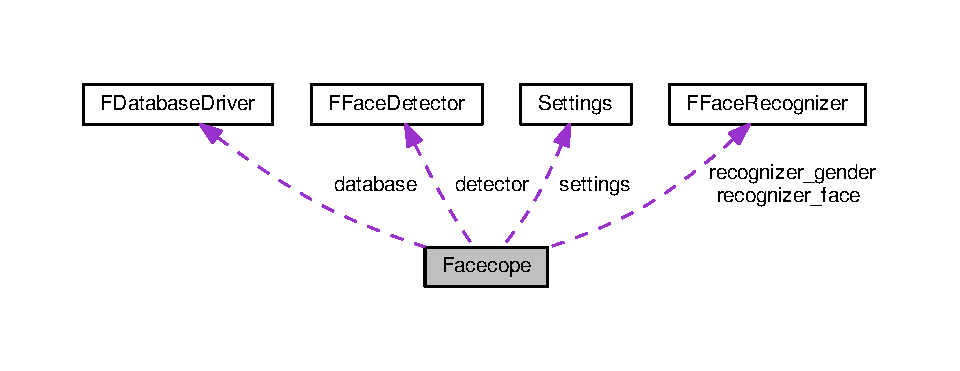
\includegraphics[width=350pt]{structFacecope__coll__graph}
\end{center}
\end{figure}
\subsection*{Public Attributes}
\begin{DoxyCompactItemize}
\item 
\mbox{\Hypertarget{structFacecope_ad609003ac3065b7eb4f8968d50a259e8}\label{structFacecope_ad609003ac3065b7eb4f8968d50a259e8}} 
\hyperlink{classFFaceDetector}{F\+Face\+Detector} $\ast$ {\bfseries detector}
\item 
\mbox{\Hypertarget{structFacecope_af097e8c7b1a1f206c7784eee1102f878}\label{structFacecope_af097e8c7b1a1f206c7784eee1102f878}} 
\hyperlink{classFFaceRecognizer}{F\+Face\+Recognizer} $\ast$ {\bfseries recognizer\+\_\+face}
\item 
\mbox{\Hypertarget{structFacecope_a04e6ee9ccdaa87c749a4ceeb33675bdf}\label{structFacecope_a04e6ee9ccdaa87c749a4ceeb33675bdf}} 
\hyperlink{classFFaceRecognizer}{F\+Face\+Recognizer} $\ast$ {\bfseries recognizer\+\_\+gender}
\item 
\mbox{\Hypertarget{structFacecope_a1789673db175e039fe9d9286d89ee1c8}\label{structFacecope_a1789673db175e039fe9d9286d89ee1c8}} 
\hyperlink{classFDatabaseDriver}{F\+Database\+Driver} $\ast$ {\bfseries database}
\item 
\mbox{\Hypertarget{structFacecope_a787a6f57e45567529433bc6f45396559}\label{structFacecope_a787a6f57e45567529433bc6f45396559}} 
\hyperlink{classSettings}{Settings} $\ast$ {\bfseries settings}
\end{DoxyCompactItemize}


The documentation for this struct was generated from the following file\+:\begin{DoxyCompactItemize}
\item 
Facecope/\+Facecope\+Core/include/\hyperlink{FacecopeTypes_8h}{Facecope\+Types.\+h}\end{DoxyCompactItemize}

\hypertarget{classFDatabaseDriver}{}\section{F\+Database\+Driver Class Reference}
\label{classFDatabaseDriver}\index{F\+Database\+Driver@{F\+Database\+Driver}}
\subsection*{Public Member Functions}
\begin{DoxyCompactItemize}
\item 
\mbox{\Hypertarget{classFDatabaseDriver_a33fa52fbcf2c2ece3a967fd0a6663dc9}\label{classFDatabaseDriver_a33fa52fbcf2c2ece3a967fd0a6663dc9}} 
{\bfseries F\+Database\+Driver} (\hyperlink{classSettings}{Settings} \&settings)
\item 
\mbox{\Hypertarget{classFDatabaseDriver_abb15fbf0aeedeee06a66ef7237667b18}\label{classFDatabaseDriver_abb15fbf0aeedeee06a66ef7237667b18}} 
Q\+Map$<$ Q\+String, Q\+Variant $>$ {\bfseries get\+\_\+user} (int id)
\item 
\mbox{\Hypertarget{classFDatabaseDriver_aa85a5aef397dee513c1c022994f77dfd}\label{classFDatabaseDriver_aa85a5aef397dee513c1c022994f77dfd}} 
Q\+String {\bfseries get} (int id, const Q\+String \&key)
\item 
\mbox{\Hypertarget{classFDatabaseDriver_a90cdca46d760181dc3ab757553e4dc26}\label{classFDatabaseDriver_a90cdca46d760181dc3ab757553e4dc26}} 
bool {\bfseries insert} (const Q\+String \&key, const Q\+String \&value)
\item 
\mbox{\Hypertarget{classFDatabaseDriver_af939b7d4d2630829eafc87d0dfb31204}\label{classFDatabaseDriver_af939b7d4d2630829eafc87d0dfb31204}} 
int {\bfseries get\+Next\+Id} ()
\item 
\mbox{\Hypertarget{classFDatabaseDriver_ad7c8cab4fab02c17fa7cbd7e95b7a9d5}\label{classFDatabaseDriver_ad7c8cab4fab02c17fa7cbd7e95b7a9d5}} 
bool {\bfseries set} (int id, const Q\+String \&key, const Q\+String \&value)
\item 
\mbox{\Hypertarget{classFDatabaseDriver_aa8e8110be5691edac0294e6b922ebe06}\label{classFDatabaseDriver_aa8e8110be5691edac0294e6b922ebe06}} 
void {\bfseries close\+Data\+Base} ()
\item 
\mbox{\Hypertarget{classFDatabaseDriver_a76c9f4db4fbf9dc5baed724fe8bbe752}\label{classFDatabaseDriver_a76c9f4db4fbf9dc5baed724fe8bbe752}} 
bool {\bfseries create\+Table} ()
\item 
\mbox{\Hypertarget{classFDatabaseDriver_a9f9447df8d67105bc2bdbefbaa9be274}\label{classFDatabaseDriver_a9f9447df8d67105bc2bdbefbaa9be274}} 
bool {\bfseries connect\+To} (const Q\+String \&path)
\end{DoxyCompactItemize}


The documentation for this class was generated from the following files\+:\begin{DoxyCompactItemize}
\item 
Facecope/\+Facecope\+Core/include/\hyperlink{FDatabaseDriver_8h}{F\+Database\+Driver.\+h}\item 
Facecope/\+Facecope\+Core/F\+Database\+Driver.\+cpp\end{DoxyCompactItemize}

\hypertarget{classFFace}{}\section{F\+Face Class Reference}
\label{classFFace}\index{F\+Face@{F\+Face}}
\subsection*{Public Member Functions}
\begin{DoxyCompactItemize}
\item 
\mbox{\Hypertarget{classFFace_a3fd9a4967475317f6992b8961ce3a70d}\label{classFFace_a3fd9a4967475317f6992b8961ce3a70d}} 
{\bfseries F\+Face} (int angle\+\_\+src, const cv\+::\+Rect \&area\+\_\+src, const cv\+::\+Rect \&eye\+\_\+1, const cv\+::\+Rect \&eye\+\_\+2, long ID=-\/1)
\item 
\mbox{\Hypertarget{classFFace_a515c08d3e3cc8e3609c549a9500938c4}\label{classFFace_a515c08d3e3cc8e3609c549a9500938c4}} 
int {\bfseries get\+\_\+rotation} ()
\item 
\mbox{\Hypertarget{classFFace_abcd3cc70544551afb7c5b44bf05d95ee}\label{classFFace_abcd3cc70544551afb7c5b44bf05d95ee}} 
cv\+::\+Rect \& {\bfseries get\+\_\+face\+\_\+frame} ()
\item 
\mbox{\Hypertarget{classFFace_afc176ac9b30f25b4b18374a4a9f996ea}\label{classFFace_afc176ac9b30f25b4b18374a4a9f996ea}} 
cv\+::\+Rect \& {\bfseries get\+\_\+original\+\_\+frame} ()
\item 
\mbox{\Hypertarget{classFFace_a3d4f56690379a92f24c2b944880b0659}\label{classFFace_a3d4f56690379a92f24c2b944880b0659}} 
long {\bfseries get\+\_\+\+ID} ()
\item 
\mbox{\Hypertarget{classFFace_a344778dae514f82c0f02776018a1718a}\label{classFFace_a344778dae514f82c0f02776018a1718a}} 
\hyperlink{structHuman}{Human} \& {\bfseries get\+\_\+info} ()
\item 
\mbox{\Hypertarget{classFFace_a6a8dd08854026cffaec7d830a25d79b1}\label{classFFace_a6a8dd08854026cffaec7d830a25d79b1}} 
\hyperlink{structEye}{Eye} \& {\bfseries get\+\_\+left\+\_\+eye} (bool normalized)
\item 
\mbox{\Hypertarget{classFFace_ab56c17cdfb69d1aba6d85a9c55d58296}\label{classFFace_ab56c17cdfb69d1aba6d85a9c55d58296}} 
\hyperlink{structEye}{Eye} \& {\bfseries get\+\_\+rigth\+\_\+eye} (bool normalized)
\item 
\mbox{\Hypertarget{classFFace_ac7b75ba2e441587ce65d08b4500b4f42}\label{classFFace_ac7b75ba2e441587ce65d08b4500b4f42}} 
int {\bfseries get\+\_\+rotation\+\_\+original} ()
\item 
\mbox{\Hypertarget{classFFace_a40ca817ea963d26cc5eb9c74cdfa1f23}\label{classFFace_a40ca817ea963d26cc5eb9c74cdfa1f23}} 
void {\bfseries set\+\_\+rotation} (int angle)
\item 
\mbox{\Hypertarget{classFFace_a797bd14396f31278615dca2be1faccbb}\label{classFFace_a797bd14396f31278615dca2be1faccbb}} 
void {\bfseries set\+\_\+original\+\_\+frame} (const cv\+::\+Rect \&frame)
\item 
\mbox{\Hypertarget{classFFace_abb6be32d9a492f09ea546634d52625cb}\label{classFFace_abb6be32d9a492f09ea546634d52625cb}} 
void {\bfseries set\+\_\+\+ID} (long ID)
\item 
\mbox{\Hypertarget{classFFace_ac9288bb881068f095d6134fac2e86932}\label{classFFace_ac9288bb881068f095d6134fac2e86932}} 
void {\bfseries create\+\_\+eyes} (const cv\+::\+Rect \&eye\+\_\+frame)
\item 
\mbox{\Hypertarget{classFFace_a1c38ba4370f0869574015386b57fd8d2}\label{classFFace_a1c38ba4370f0869574015386b57fd8d2}} 
void {\bfseries set\+\_\+eyes} (const cv\+::\+Rect \&eye\+\_\+frame\+\_\+1, const cv\+::\+Rect \&eye\+\_\+frame\+\_\+2)
\item 
\mbox{\Hypertarget{classFFace_a58e3df53a38092ee907f83d4f906163b}\label{classFFace_a58e3df53a38092ee907f83d4f906163b}} 
void {\bfseries set\+\_\+info} (const \hyperlink{structHuman}{Human} \&human)
\end{DoxyCompactItemize}


The documentation for this class was generated from the following files\+:\begin{DoxyCompactItemize}
\item 
Facecope/\+Facecope\+Core/include/F\+Face.\+h\item 
Facecope/\+Facecope\+Core/F\+Face.\+cpp\end{DoxyCompactItemize}

\hypertarget{classFFaceDetector}{}\section{F\+Face\+Detector Class Reference}
\label{classFFaceDetector}\index{F\+Face\+Detector@{F\+Face\+Detector}}
\subsection*{Public Member Functions}
\begin{DoxyCompactItemize}
\item 
\mbox{\Hypertarget{classFFaceDetector_a85d71ee3f97ea60bcd7adc94d68d30e6}\label{classFFaceDetector_a85d71ee3f97ea60bcd7adc94d68d30e6}} 
{\bfseries F\+Face\+Detector} (const std\+::string \&cascades\+Dir\+\_\+face\+\_\+haar=C\+A\+S\+C\+A\+D\+E\+\_\+\+F\+A\+C\+E\+\_\+\+H\+A\+A\+R\+\_\+\+P\+A\+TH, const std\+::string \&cascades\+Dir\+\_\+face\+\_\+lbp=C\+A\+S\+C\+A\+D\+E\+\_\+\+F\+A\+C\+E\+\_\+\+L\+B\+P\+\_\+\+P\+A\+TH, const std\+::string \&cascades\+Dir\+\_\+eye\+\_\+haar=C\+A\+S\+C\+A\+D\+E\+\_\+\+E\+Y\+E\+S\+\_\+\+H\+A\+A\+R\+\_\+\+P\+A\+TH)
\item 
\mbox{\Hypertarget{classFFaceDetector_a734d9d1224a97db0db4556e2804bb04c}\label{classFFaceDetector_a734d9d1224a97db0db4556e2804bb04c}} 
void {\bfseries detect\+\_\+faces} (\hyperlink{classFImage}{F\+Image} \&image, bool remove\+Face\+Without\+Eye=false, int cascade\+\_\+type=H\+A\+AR, int steps=0, int angle\+\_\+range=360, double scale\+Factor=1.\+2, cv\+::\+Size min\+\_\+size\+\_\+ratio=cv\+::\+Size(), cv\+::\+Size max\+\_\+size\+\_\+ratio=cv\+::\+Size())
\item 
\mbox{\Hypertarget{classFFaceDetector_a6bf029be40508d735d440f193083d2a9}\label{classFFaceDetector_a6bf029be40508d735d440f193083d2a9}} 
void {\bfseries detect\+\_\+faces} (const cv\+::\+Mat \&image, std\+::vector$<$ \hyperlink{classFFace}{F\+Face} $\ast$$>$ \&faces, bool remove\+Face\+Without\+Eye=false, int cascade\+\_\+type=H\+A\+AR, int steps=0, int angle\+\_\+range=360, double scale\+Factor=1.\+2, cv\+::\+Size min\+\_\+size\+\_\+ratio=cv\+::\+Size(), cv\+::\+Size max\+\_\+size\+\_\+ratio=cv\+::\+Size())
\item 
\mbox{\Hypertarget{classFFaceDetector_a1799777797a5153b50b40615ae58e953}\label{classFFaceDetector_a1799777797a5153b50b40615ae58e953}} 
bool {\bfseries is\+Loaded} (int what)
\end{DoxyCompactItemize}


The documentation for this class was generated from the following files\+:\begin{DoxyCompactItemize}
\item 
Facecope/\+Facecope\+Core/include/F\+Face\+Detector.\+h\item 
Facecope/\+Facecope\+Core/F\+Face\+Detector.\+cpp\end{DoxyCompactItemize}

\hypertarget{classFFaceModel}{}\section{F\+Face\+Model Class Reference}
\label{classFFaceModel}\index{F\+Face\+Model@{F\+Face\+Model}}


Inheritance diagram for F\+Face\+Model\+:
\nopagebreak
\begin{figure}[H]
\begin{center}
\leavevmode
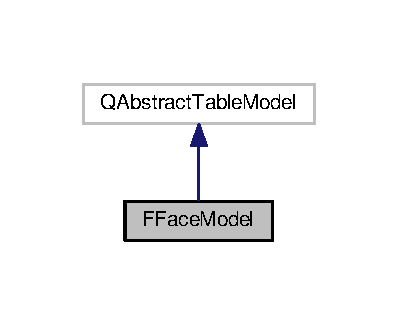
\includegraphics[width=191pt]{classFFaceModel__inherit__graph}
\end{center}
\end{figure}


Collaboration diagram for F\+Face\+Model\+:
\nopagebreak
\begin{figure}[H]
\begin{center}
\leavevmode
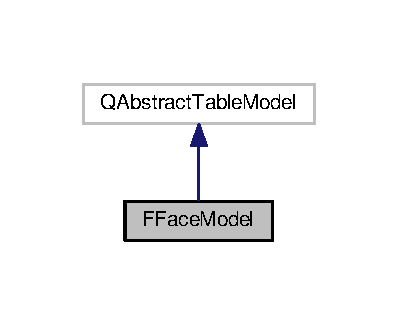
\includegraphics[width=191pt]{classFFaceModel__coll__graph}
\end{center}
\end{figure}
\subsection*{Public Slots}
\begin{DoxyCompactItemize}
\item 
\mbox{\Hypertarget{classFFaceModel_adcef175f955952d2818af98f2a3d7df0}\label{classFFaceModel_adcef175f955952d2818af98f2a3d7df0}} 
void {\bfseries set\+\_\+image\+\_\+size} (const Q\+Size \&new\+Size)
\end{DoxyCompactItemize}
\subsection*{Public Member Functions}
\begin{DoxyCompactItemize}
\item 
\mbox{\Hypertarget{classFFaceModel_a78b485cf9ab083b02b589216738ec1c1}\label{classFFaceModel_a78b485cf9ab083b02b589216738ec1c1}} 
{\bfseries F\+Face\+Model} (\hyperlink{structFacecope}{Facecope} \&facecope, \hyperlink{classFImage}{F\+Image} \&f\+\_\+image, Q\+Object $\ast$parent=0)
\item 
\mbox{\Hypertarget{classFFaceModel_af3cd862738b4abe440dd7cd740931982}\label{classFFaceModel_af3cd862738b4abe440dd7cd740931982}} 
int {\bfseries row\+Count} (const Q\+Model\+Index \&parent=Q\+Model\+Index()) const override
\item 
\mbox{\Hypertarget{classFFaceModel_a1efe53f446828417b8f7c39030e9a4ac}\label{classFFaceModel_a1efe53f446828417b8f7c39030e9a4ac}} 
int {\bfseries column\+Count} (const Q\+Model\+Index \&parent=Q\+Model\+Index()) const override
\item 
\mbox{\Hypertarget{classFFaceModel_a7cee177081f026c5e01cd164859c5275}\label{classFFaceModel_a7cee177081f026c5e01cd164859c5275}} 
Q\+Variant {\bfseries data} (const Q\+Model\+Index \&index, int role=Qt\+::\+Display\+Role) const override
\item 
\mbox{\Hypertarget{classFFaceModel_a328af9e0b4af2a6187bff82de4ab2bd7}\label{classFFaceModel_a328af9e0b4af2a6187bff82de4ab2bd7}} 
Q\+Variant {\bfseries header\+Data} (int section, Qt\+::\+Orientation orientation, int role=Qt\+::\+Display\+Role) const
\item 
\mbox{\Hypertarget{classFFaceModel_a2ac11aefcdfdbf400d945ce9d99e0893}\label{classFFaceModel_a2ac11aefcdfdbf400d945ce9d99e0893}} 
\hyperlink{classFFace}{F\+Face} $\ast$ {\bfseries get\+\_\+item} (int row)
\item 
\mbox{\Hypertarget{classFFaceModel_ae494a0f8028db819b579aea2ce0c1074}\label{classFFaceModel_ae494a0f8028db819b579aea2ce0c1074}} 
\hyperlink{classFImage}{F\+Image} $\ast$ {\bfseries get\+\_\+image} ()
\end{DoxyCompactItemize}


The documentation for this class was generated from the following files\+:\begin{DoxyCompactItemize}
\item 
Facecope/models/include/F\+Face\+Model.\+h\item 
Facecope/models/F\+Face\+Model.\+cpp\end{DoxyCompactItemize}

\hypertarget{classFFaceRecognizer}{}\section{F\+Face\+Recognizer Class Reference}
\label{classFFaceRecognizer}\index{F\+Face\+Recognizer@{F\+Face\+Recognizer}}
\subsection*{Public Member Functions}
\begin{DoxyCompactItemize}
\item 
\mbox{\Hypertarget{classFFaceRecognizer_ae6cbd9976fcef82a1810c900461e4324}\label{classFFaceRecognizer_ae6cbd9976fcef82a1810c900461e4324}} 
{\bfseries F\+Face\+Recognizer} (const std\+::string \&dir\+Path, const cv\+::\+Size \&size\+Of\+Image=cv\+::\+Size(150, 150), int num\+Of\+Components=80, double threahold=D\+B\+L\+\_\+\+M\+AX)
\item 
\mbox{\Hypertarget{classFFaceRecognizer_af53533828fa55959003de034ce36f5bc}\label{classFFaceRecognizer_af53533828fa55959003de034ce36f5bc}} 
{\bfseries F\+Face\+Recognizer} (const cv\+::\+Size \&image\+Scale\+Size=cv\+::\+Size(150, 150))
\item 
\mbox{\Hypertarget{classFFaceRecognizer_aa115a2ee94b62ba56c24677681d90cf5}\label{classFFaceRecognizer_aa115a2ee94b62ba56c24677681d90cf5}} 
int {\bfseries recognize} (const cv\+::\+Mat \&face)
\item 
\mbox{\Hypertarget{classFFaceRecognizer_aad62aeda81f1f80a1474a8c4b7cdffa6}\label{classFFaceRecognizer_aad62aeda81f1f80a1474a8c4b7cdffa6}} 
bool {\bfseries load} (const std\+::string \&load\+Path)
\item 
\mbox{\Hypertarget{classFFaceRecognizer_a69dc6bf3209b3e8b46e0315682281ada}\label{classFFaceRecognizer_a69dc6bf3209b3e8b46e0315682281ada}} 
bool {\bfseries save} (const std\+::string \&save\+Path)
\item 
\mbox{\Hypertarget{classFFaceRecognizer_a281e25216015de853e1cf01689e13d9c}\label{classFFaceRecognizer_a281e25216015de853e1cf01689e13d9c}} 
void {\bfseries set\+\_\+threahold} (double threahold)
\item 
\mbox{\Hypertarget{classFFaceRecognizer_a2e482df0822dc7747ef5cff0a31b75a8}\label{classFFaceRecognizer_a2e482df0822dc7747ef5cff0a31b75a8}} 
double {\bfseries get\+\_\+threahold} ()
\item 
\mbox{\Hypertarget{classFFaceRecognizer_aeead25d21c46e87d6895fb63a80a084f}\label{classFFaceRecognizer_aeead25d21c46e87d6895fb63a80a084f}} 
int {\bfseries get\+\_\+num\+\_\+of\+\_\+components} ()
\item 
\mbox{\Hypertarget{classFFaceRecognizer_ae26c8de753c3a5c48b2270d1e80d769c}\label{classFFaceRecognizer_ae26c8de753c3a5c48b2270d1e80d769c}} 
void {\bfseries set\+\_\+num\+\_\+of\+\_\+components} (int number)
\item 
\mbox{\Hypertarget{classFFaceRecognizer_ad8d59cc8cd95ee58877b49f59bfbc48a}\label{classFFaceRecognizer_ad8d59cc8cd95ee58877b49f59bfbc48a}} 
bool {\bfseries learn} (const std\+::vector$<$ cv\+::\+Mat $>$ \&images, const std\+::vector$<$ int $>$ labels)
\item 
\mbox{\Hypertarget{classFFaceRecognizer_a417ead8d39d07d5b1cbfc5b8ac95f014}\label{classFFaceRecognizer_a417ead8d39d07d5b1cbfc5b8ac95f014}} 
cv\+::\+Size {\bfseries get\+\_\+size\+\_\+of\+\_\+image} ()
\end{DoxyCompactItemize}


The documentation for this class was generated from the following files\+:\begin{DoxyCompactItemize}
\item 
Facecope/\+Facecope\+Core/include/F\+Face\+Recognizer.\+h\item 
Facecope/\+Facecope\+Core/F\+Face\+Recognizer.\+cpp\end{DoxyCompactItemize}

\hypertarget{classFHelpWidget}{}\section{F\+Help\+Widget Class Reference}
\label{classFHelpWidget}\index{F\+Help\+Widget@{F\+Help\+Widget}}


Inheritance diagram for F\+Help\+Widget\+:
\nopagebreak
\begin{figure}[H]
\begin{center}
\leavevmode
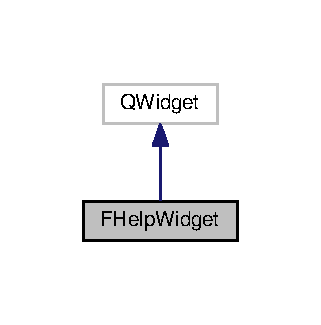
\includegraphics[width=154pt]{classFHelpWidget__inherit__graph}
\end{center}
\end{figure}


Collaboration diagram for F\+Help\+Widget\+:
\nopagebreak
\begin{figure}[H]
\begin{center}
\leavevmode
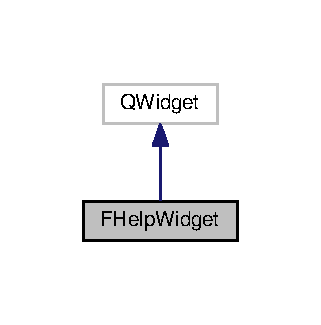
\includegraphics[width=154pt]{classFHelpWidget__coll__graph}
\end{center}
\end{figure}
\subsection*{Public Member Functions}
\begin{DoxyCompactItemize}
\item 
\mbox{\Hypertarget{classFHelpWidget_aa30f30781babf7d9ba69a72ca7830fcf}\label{classFHelpWidget_aa30f30781babf7d9ba69a72ca7830fcf}} 
{\bfseries F\+Help\+Widget} (Q\+Widget $\ast$parent=0)
\end{DoxyCompactItemize}


The documentation for this class was generated from the following files\+:\begin{DoxyCompactItemize}
\item 
Facecope/widgets/include/\hyperlink{FHelpWidget_8h}{F\+Help\+Widget.\+h}\item 
Facecope/widgets/F\+Help\+Widget.\+cpp\end{DoxyCompactItemize}

\hypertarget{classFImage}{}\section{F\+Image Class Reference}
\label{classFImage}\index{F\+Image@{F\+Image}}
\subsection*{Public Member Functions}
\begin{DoxyCompactItemize}
\item 
\mbox{\Hypertarget{classFImage_ab0b48ac01caee473e5e4363274f4e166}\label{classFImage_ab0b48ac01caee473e5e4363274f4e166}} 
{\bfseries F\+Image} (const Q\+String \&path)
\item 
\mbox{\Hypertarget{classFImage_abd1c56744d46d6d7cc559d902532f9e2}\label{classFImage_abd1c56744d46d6d7cc559d902532f9e2}} 
{\bfseries F\+Image} (const cv\+::\+Mat \&mat)
\item 
\mbox{\Hypertarget{classFImage_a5769ad6633c2f37fb5f13c4b552bb8ed}\label{classFImage_a5769ad6633c2f37fb5f13c4b552bb8ed}} 
Q\+String {\bfseries get\+\_\+name} () const
\item 
\mbox{\Hypertarget{classFImage_ac14200c10a9a112ee92792c2958ec710}\label{classFImage_ac14200c10a9a112ee92792c2958ec710}} 
void {\bfseries set\+\_\+name} (const Q\+String \&name)
\item 
\mbox{\Hypertarget{classFImage_a82cab8d4bf02ed4e316bcbafd7503bb6}\label{classFImage_a82cab8d4bf02ed4e316bcbafd7503bb6}} 
Q\+Image {\bfseries to\+\_\+q\+\_\+image} ()
\item 
\mbox{\Hypertarget{classFImage_ac20f0314cc27a646f7c051ed30521791}\label{classFImage_ac20f0314cc27a646f7c051ed30521791}} 
cv\+::\+Mat {\bfseries to\+\_\+cv\+\_\+image} ()
\item 
\mbox{\Hypertarget{classFImage_a6ddf652e7426034db1928ab6f712ffe1}\label{classFImage_a6ddf652e7426034db1928ab6f712ffe1}} 
void {\bfseries set\+\_\+recognized} (bool recognized, double threahold\+\_\+of\+\_\+recognition)
\item 
\mbox{\Hypertarget{classFImage_a552d285fc2e3af631a62f0919a445c62}\label{classFImage_a552d285fc2e3af631a62f0919a445c62}} 
void {\bfseries set\+\_\+detected} (bool detected, int steps)
\item 
\mbox{\Hypertarget{classFImage_a9df7dccbbfedc6fcd0d9277b9d84da04}\label{classFImage_a9df7dccbbfedc6fcd0d9277b9d84da04}} 
int {\bfseries add\+\_\+face} (\hyperlink{classFFace}{F\+Face} $\ast$face)
\item 
\mbox{\Hypertarget{classFImage_a6075a7daf1825d3b36d48a1cab394528}\label{classFImage_a6075a7daf1825d3b36d48a1cab394528}} 
void {\bfseries add\+\_\+faces} (std\+::vector$<$ \hyperlink{classFFace}{F\+Face} $\ast$$>$ \&faces)
\item 
\mbox{\Hypertarget{classFImage_a929e98398242b5c90b89189d4dc8e6e3}\label{classFImage_a929e98398242b5c90b89189d4dc8e6e3}} 
\hyperlink{classFFace}{F\+Face} $\ast$ {\bfseries remove\+\_\+face} (long ID)
\item 
\mbox{\Hypertarget{classFImage_a106c5f6eb73bb7f9688f986c8648f8d1}\label{classFImage_a106c5f6eb73bb7f9688f986c8648f8d1}} 
Q\+Vector$<$ \hyperlink{classFFace}{F\+Face} $\ast$ $>$ \& {\bfseries get\+\_\+faces} ()
\item 
\mbox{\Hypertarget{classFImage_a4b5522340534c0cdb89c1f33734626ab}\label{classFImage_a4b5522340534c0cdb89c1f33734626ab}} 
\hyperlink{classFFace}{F\+Face} $\ast$ {\bfseries get\+\_\+face} (long ID)
\item 
\mbox{\Hypertarget{classFImage_a6a103bfcb9e83c062dd5ae8ede68cab9}\label{classFImage_a6a103bfcb9e83c062dd5ae8ede68cab9}} 
void {\bfseries clear} ()
\item 
\mbox{\Hypertarget{classFImage_a82d60358d733dce9caef827a17928bc5}\label{classFImage_a82d60358d733dce9caef827a17928bc5}} 
bool {\bfseries empty} () const
\item 
\mbox{\Hypertarget{classFImage_adf4496205cd140b3410cdabcfe40d5ae}\label{classFImage_adf4496205cd140b3410cdabcfe40d5ae}} 
cv\+::\+Size {\bfseries cv\+\_\+size} () const
\item 
\mbox{\Hypertarget{classFImage_a799b0c83add0d9dee24b192c587596ed}\label{classFImage_a799b0c83add0d9dee24b192c587596ed}} 
Q\+Size {\bfseries q\+\_\+size} () const
\item 
\mbox{\Hypertarget{classFImage_a721d1e114f45d53d50296bfe2e22f41f}\label{classFImage_a721d1e114f45d53d50296bfe2e22f41f}} 
bool {\bfseries contains} (int val)
\item 
\mbox{\Hypertarget{classFImage_a4c6d99e648fbd7a107337b6bd2991012}\label{classFImage_a4c6d99e648fbd7a107337b6bd2991012}} 
cv\+::\+Mat {\bfseries get\+\_\+face\+\_\+cv\+\_\+image} (\hyperlink{classFFace}{F\+Face} $\ast$face)
\item 
\mbox{\Hypertarget{classFImage_a0edb8f7b81d65d7d28e22f1417a601df}\label{classFImage_a0edb8f7b81d65d7d28e22f1417a601df}} 
Q\+Rect {\bfseries get\+\_\+face\+\_\+q\+\_\+frame} (\hyperlink{classFFace}{F\+Face} $\ast$face)
\item 
\mbox{\Hypertarget{classFImage_aa00488f14f8f8c8ea49f27a7f26a0a6b}\label{classFImage_aa00488f14f8f8c8ea49f27a7f26a0a6b}} 
bool {\bfseries is\+Recognized} () const
\item 
\mbox{\Hypertarget{classFImage_a3a9633f8b7b7c0f64520770135c518b4}\label{classFImage_a3a9633f8b7b7c0f64520770135c518b4}} 
bool {\bfseries is\+Detected} () const
\item 
\mbox{\Hypertarget{classFImage_aeb31036059d0c85596118019d4ba8b5c}\label{classFImage_aeb31036059d0c85596118019d4ba8b5c}} 
int {\bfseries get\+Detection\+\_\+steps} () const
\item 
\mbox{\Hypertarget{classFImage_acc32b56d339159ba4e8a6a16fd25e375}\label{classFImage_acc32b56d339159ba4e8a6a16fd25e375}} 
double {\bfseries get\+Threahold\+\_\+of\+\_\+recognition} () const
\end{DoxyCompactItemize}


The documentation for this class was generated from the following files\+:\begin{DoxyCompactItemize}
\item 
Facecope/\+Facecope\+Core/include/\hyperlink{FImage_8h}{F\+Image.\+h}\item 
Facecope/\+Facecope\+Core/F\+Image.\+cpp\end{DoxyCompactItemize}

\hypertarget{classFImageDrawAreaWidget}{}\section{F\+Image\+Draw\+Area\+Widget Class Reference}
\label{classFImageDrawAreaWidget}\index{F\+Image\+Draw\+Area\+Widget@{F\+Image\+Draw\+Area\+Widget}}


Inheritance diagram for F\+Image\+Draw\+Area\+Widget\+:
\nopagebreak
\begin{figure}[H]
\begin{center}
\leavevmode
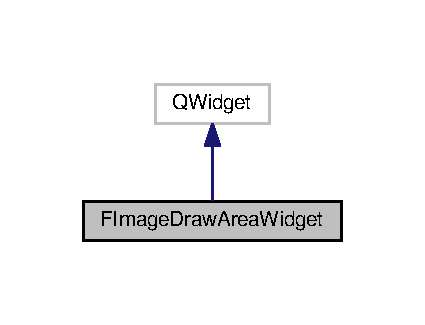
\includegraphics[width=204pt]{classFImageDrawAreaWidget__inherit__graph}
\end{center}
\end{figure}


Collaboration diagram for F\+Image\+Draw\+Area\+Widget\+:
\nopagebreak
\begin{figure}[H]
\begin{center}
\leavevmode
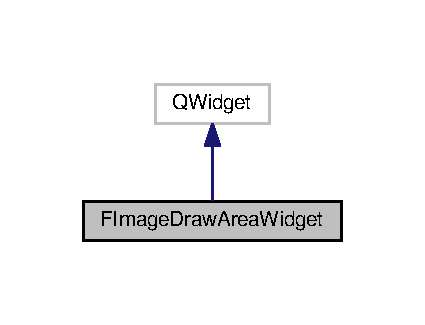
\includegraphics[width=204pt]{classFImageDrawAreaWidget__coll__graph}
\end{center}
\end{figure}
\subsection*{Public Member Functions}
\begin{DoxyCompactItemize}
\item 
\mbox{\Hypertarget{classFImageDrawAreaWidget_a7abc8014326256d81eb71e2296ed28b3}\label{classFImageDrawAreaWidget_a7abc8014326256d81eb71e2296ed28b3}} 
{\bfseries F\+Image\+Draw\+Area\+Widget} (\hyperlink{structFacecope}{Facecope} \&facecope, \hyperlink{classFImage}{F\+Image} \&image, Q\+Widget $\ast$parent=0)
\item 
\mbox{\Hypertarget{classFImageDrawAreaWidget_a137ca0e7a4ed84e42dccc554f62f2e23}\label{classFImageDrawAreaWidget_a137ca0e7a4ed84e42dccc554f62f2e23}} 
Q\+Size {\bfseries minimum\+Size\+Hint} () const override
\item 
\mbox{\Hypertarget{classFImageDrawAreaWidget_a184db264e0f07a783009b77bc7f6f17d}\label{classFImageDrawAreaWidget_a184db264e0f07a783009b77bc7f6f17d}} 
Q\+Size {\bfseries size\+Hint} () const override
\end{DoxyCompactItemize}
\subsection*{Protected Member Functions}
\begin{DoxyCompactItemize}
\item 
\mbox{\Hypertarget{classFImageDrawAreaWidget_a8b393488d7169477e5c14c708a22ace3}\label{classFImageDrawAreaWidget_a8b393488d7169477e5c14c708a22ace3}} 
void {\bfseries paint\+Event} (Q\+Paint\+Event $\ast$event) override
\end{DoxyCompactItemize}


The documentation for this class was generated from the following files\+:\begin{DoxyCompactItemize}
\item 
Facecope/widgets/include/\hyperlink{FImageDrawAreaWidget_8h}{F\+Image\+Draw\+Area\+Widget.\+h}\item 
Facecope/widgets/F\+Image\+Draw\+Area\+Widget.\+cpp\end{DoxyCompactItemize}

\hypertarget{classFImageProxyModel}{}\section{F\+Image\+Proxy\+Model Class Reference}
\label{classFImageProxyModel}\index{F\+Image\+Proxy\+Model@{F\+Image\+Proxy\+Model}}


Inheritance diagram for F\+Image\+Proxy\+Model\+:
\nopagebreak
\begin{figure}[H]
\begin{center}
\leavevmode
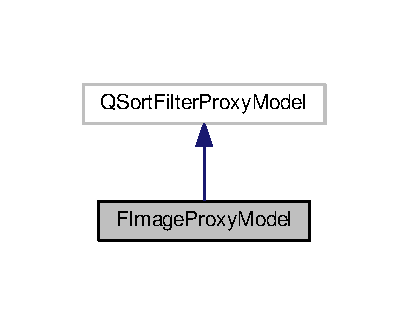
\includegraphics[width=196pt]{classFImageProxyModel__inherit__graph}
\end{center}
\end{figure}


Collaboration diagram for F\+Image\+Proxy\+Model\+:
\nopagebreak
\begin{figure}[H]
\begin{center}
\leavevmode
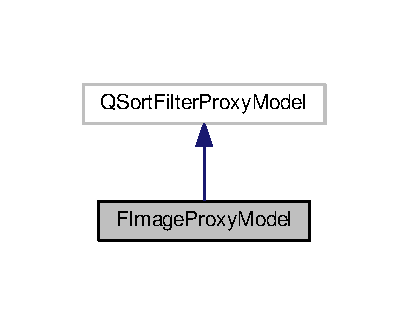
\includegraphics[width=196pt]{classFImageProxyModel__coll__graph}
\end{center}
\end{figure}
\subsection*{Public Slots}
\begin{DoxyCompactItemize}
\item 
\mbox{\Hypertarget{classFImageProxyModel_a5a10355cb8221903eb2c008d8d6757b2}\label{classFImageProxyModel_a5a10355cb8221903eb2c008d8d6757b2}} 
void {\bfseries clear} ()
\item 
\mbox{\Hypertarget{classFImageProxyModel_ae34e7bb126cbc6d36214655a80e1246f}\label{classFImageProxyModel_ae34e7bb126cbc6d36214655a80e1246f}} 
void {\bfseries set\+Show\+\_\+recognized} (bool value)
\item 
\mbox{\Hypertarget{classFImageProxyModel_ad6908944746afd07f2caf0d1f665db85}\label{classFImageProxyModel_ad6908944746afd07f2caf0d1f665db85}} 
void {\bfseries set\+Show\+\_\+unrecognized} (bool value)
\item 
\mbox{\Hypertarget{classFImageProxyModel_ae9db9cd4784521a8384351d8b330ec4d}\label{classFImageProxyModel_ae9db9cd4784521a8384351d8b330ec4d}} 
void {\bfseries set\+Show\+\_\+without\+\_\+human} (bool value)
\item 
\mbox{\Hypertarget{classFImageProxyModel_aef7f4ed60085955e6264cbfdbbd49b41}\label{classFImageProxyModel_aef7f4ed60085955e6264cbfdbbd49b41}} 
void {\bfseries set\+Show\+\_\+only\+\_\+human} (bool value)
\item 
\mbox{\Hypertarget{classFImageProxyModel_a3e65daf7d2cc0115bac7e7920c91df9e}\label{classFImageProxyModel_a3e65daf7d2cc0115bac7e7920c91df9e}} 
void {\bfseries set\+Min\+\_\+human\+\_\+number} (int value)
\item 
\mbox{\Hypertarget{classFImageProxyModel_a8a29d8f0b3ac2a9693d3ca47f718151e}\label{classFImageProxyModel_a8a29d8f0b3ac2a9693d3ca47f718151e}} 
void {\bfseries apply} ()
\end{DoxyCompactItemize}
\subsection*{Public Member Functions}
\begin{DoxyCompactItemize}
\item 
\mbox{\Hypertarget{classFImageProxyModel_a00dd19eaa241d81f83b5d827049b4ba8}\label{classFImageProxyModel_a00dd19eaa241d81f83b5d827049b4ba8}} 
{\bfseries F\+Image\+Proxy\+Model} (\hyperlink{classFMainFacecopeModel}{F\+Main\+Facecope\+Model} \&src\+\_\+model, Q\+Object $\ast$parent=0)
\item 
\mbox{\Hypertarget{classFImageProxyModel_aa684f4c8e2eb18a1ed29e57de9f1c5ba}\label{classFImageProxyModel_aa684f4c8e2eb18a1ed29e57de9f1c5ba}} 
bool {\bfseries filter\+Accepts\+Row} (int source\+\_\+row, const Q\+Model\+Index \&source\+\_\+parent) const
\item 
\mbox{\Hypertarget{classFImageProxyModel_aa3fba9a128badc5c4b06a0a4caafa4c2}\label{classFImageProxyModel_aa3fba9a128badc5c4b06a0a4caafa4c2}} 
int {\bfseries get\+Displaing\+Photos} ()
\end{DoxyCompactItemize}


The documentation for this class was generated from the following files\+:\begin{DoxyCompactItemize}
\item 
Facecope/models/include/\hyperlink{FImageProxyModel_8h}{F\+Image\+Proxy\+Model.\+h}\item 
Facecope/models/F\+Image\+Proxy\+Model.\+cpp\end{DoxyCompactItemize}

\hypertarget{classFImageShowDialog}{}\section{F\+Image\+Show\+Dialog Class Reference}
\label{classFImageShowDialog}\index{F\+Image\+Show\+Dialog@{F\+Image\+Show\+Dialog}}


Inheritance diagram for F\+Image\+Show\+Dialog\+:
\nopagebreak
\begin{figure}[H]
\begin{center}
\leavevmode
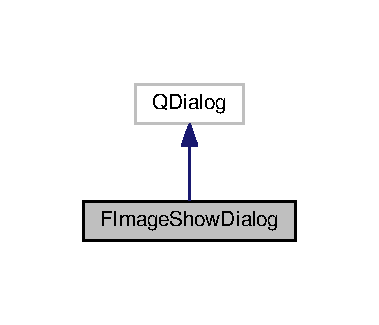
\includegraphics[width=182pt]{classFImageShowDialog__inherit__graph}
\end{center}
\end{figure}


Collaboration diagram for F\+Image\+Show\+Dialog\+:
\nopagebreak
\begin{figure}[H]
\begin{center}
\leavevmode
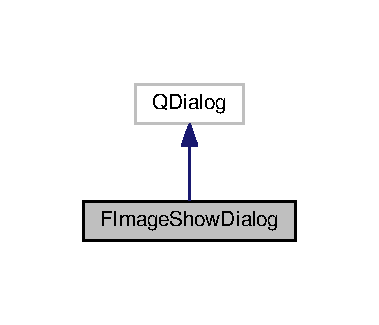
\includegraphics[width=182pt]{classFImageShowDialog__coll__graph}
\end{center}
\end{figure}
\subsection*{Public Member Functions}
\begin{DoxyCompactItemize}
\item 
\mbox{\Hypertarget{classFImageShowDialog_a4c7b77746ae11fe69bdca3262b311c5a}\label{classFImageShowDialog_a4c7b77746ae11fe69bdca3262b311c5a}} 
{\bfseries F\+Image\+Show\+Dialog} (\hyperlink{structFacecope}{Facecope} \&facecope, \hyperlink{classFImage}{F\+Image} \&image, Q\+Widget $\ast$parent=0)
\end{DoxyCompactItemize}


The documentation for this class was generated from the following files\+:\begin{DoxyCompactItemize}
\item 
Facecope/widgets/include/\hyperlink{FImageShowDialog_8h}{F\+Image\+Show\+Dialog.\+h}\item 
Facecope/widgets/F\+Image\+Show\+Dialog.\+cpp\end{DoxyCompactItemize}

\hypertarget{classFMainFacecopeModel}{}\section{F\+Main\+Facecope\+Model Class Reference}
\label{classFMainFacecopeModel}\index{F\+Main\+Facecope\+Model@{F\+Main\+Facecope\+Model}}


Inheritance diagram for F\+Main\+Facecope\+Model\+:
\nopagebreak
\begin{figure}[H]
\begin{center}
\leavevmode
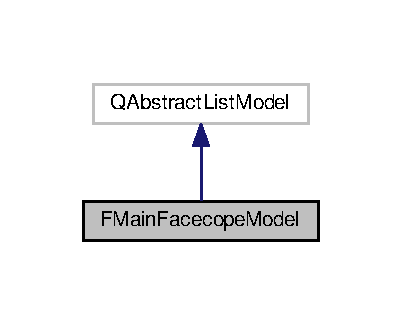
\includegraphics[width=193pt]{classFMainFacecopeModel__inherit__graph}
\end{center}
\end{figure}


Collaboration diagram for F\+Main\+Facecope\+Model\+:
\nopagebreak
\begin{figure}[H]
\begin{center}
\leavevmode
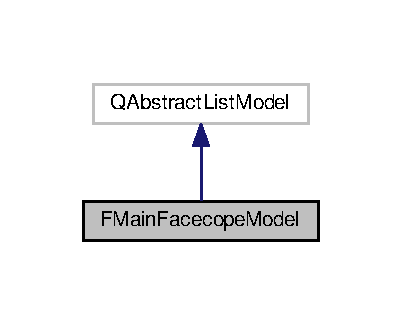
\includegraphics[width=193pt]{classFMainFacecopeModel__coll__graph}
\end{center}
\end{figure}
\subsection*{Public Slots}
\begin{DoxyCompactItemize}
\item 
\mbox{\Hypertarget{classFMainFacecopeModel_aa2377ed7d59faa527c01161500c1a18d}\label{classFMainFacecopeModel_aa2377ed7d59faa527c01161500c1a18d}} 
void {\bfseries slot\+\_\+set\+\_\+image\+\_\+size} (const Q\+Size \&new\+Size)
\item 
\mbox{\Hypertarget{classFMainFacecopeModel_a8c639e2873a4e433b30575d8cfc1d660}\label{classFMainFacecopeModel_a8c639e2873a4e433b30575d8cfc1d660}} 
void {\bfseries slot\+\_\+clear} ()
\item 
\mbox{\Hypertarget{classFMainFacecopeModel_abba3d83f3b85760d28d5c878ce646e7c}\label{classFMainFacecopeModel_abba3d83f3b85760d28d5c878ce646e7c}} 
void {\bfseries slot\+\_\+recognize} (int row)
\item 
\mbox{\Hypertarget{classFMainFacecopeModel_a22d8ffec6b8cdafa8cea02032dfd0203}\label{classFMainFacecopeModel_a22d8ffec6b8cdafa8cea02032dfd0203}} 
void {\bfseries slot\+\_\+detect} (int row)
\end{DoxyCompactItemize}
\subsection*{Public Member Functions}
\begin{DoxyCompactItemize}
\item 
\mbox{\Hypertarget{classFMainFacecopeModel_a978bd3890e0639437639d1c3a93c8f92}\label{classFMainFacecopeModel_a978bd3890e0639437639d1c3a93c8f92}} 
{\bfseries F\+Main\+Facecope\+Model} (\hyperlink{structFacecope}{Facecope} \&facecope, Q\+Object $\ast$parent=0)
\item 
\mbox{\Hypertarget{classFMainFacecopeModel_a2963e38095e5b333887d5e40a29e97c4}\label{classFMainFacecopeModel_a2963e38095e5b333887d5e40a29e97c4}} 
int {\bfseries row\+Count} (const Q\+Model\+Index \&parent=Q\+Model\+Index()) const override
\item 
\mbox{\Hypertarget{classFMainFacecopeModel_aed374733f42dc4431adae47c67a5c536}\label{classFMainFacecopeModel_aed374733f42dc4431adae47c67a5c536}} 
Q\+Variant {\bfseries data} (const Q\+Model\+Index \&index, int role=Qt\+::\+Display\+Role) const override
\item 
\mbox{\Hypertarget{classFMainFacecopeModel_ae1554769d52e9759c3d083014490b9e5}\label{classFMainFacecopeModel_ae1554769d52e9759c3d083014490b9e5}} 
bool {\bfseries remove\+Row} (int row, const Q\+Model\+Index \&parent=Q\+Model\+Index())
\item 
\mbox{\Hypertarget{classFMainFacecopeModel_aa7044acf807fae60da413b23d127ae9f}\label{classFMainFacecopeModel_aa7044acf807fae60da413b23d127ae9f}} 
const Q\+Map$<$ Q\+String, \hyperlink{classFImage}{F\+Image} $\ast$ $>$ \& {\bfseries get\+\_\+items} ()
\item 
\mbox{\Hypertarget{classFMainFacecopeModel_a1e252ebb83462b92197d5dc69262007d}\label{classFMainFacecopeModel_a1e252ebb83462b92197d5dc69262007d}} 
bool {\bfseries load} (const Q\+String \&path)
\item 
\mbox{\Hypertarget{classFMainFacecopeModel_a0c6aa5e8a388759a1c6c81d4e98ce903}\label{classFMainFacecopeModel_a0c6aa5e8a388759a1c6c81d4e98ce903}} 
bool {\bfseries remove} (const Q\+String \&key)
\item 
\mbox{\Hypertarget{classFMainFacecopeModel_acf3adfcfe3736363aee73856dc1fa142}\label{classFMainFacecopeModel_acf3adfcfe3736363aee73856dc1fa142}} 
bool {\bfseries remove} (int index)
\item 
\mbox{\Hypertarget{classFMainFacecopeModel_a9e181078dac81a412706a76f86b0bcce}\label{classFMainFacecopeModel_a9e181078dac81a412706a76f86b0bcce}} 
bool {\bfseries is\+Valid\+\_\+path} (const Q\+String \&key)
\item 
\mbox{\Hypertarget{classFMainFacecopeModel_acf65e2eb6cd2ebd5f1ddc448de077a04}\label{classFMainFacecopeModel_acf65e2eb6cd2ebd5f1ddc448de077a04}} 
\hyperlink{classFImage}{F\+Image} $\ast$ {\bfseries get\+\_\+item} (const Q\+String \&path)
\item 
\mbox{\Hypertarget{classFMainFacecopeModel_aef457c2256cfa706fb1dd98bf7106c45}\label{classFMainFacecopeModel_aef457c2256cfa706fb1dd98bf7106c45}} 
\hyperlink{classFImage}{F\+Image} $\ast$ {\bfseries get\+\_\+item} (int index)
\item 
\mbox{\Hypertarget{classFMainFacecopeModel_af0ed30ded3f6f2006d2e24ba1a5f8cb1}\label{classFMainFacecopeModel_af0ed30ded3f6f2006d2e24ba1a5f8cb1}} 
Q\+String\+List {\bfseries get\+\_\+paths} ()
\item 
\mbox{\Hypertarget{classFMainFacecopeModel_aec85665ecd3eab4e6afb0c1f235e9ab5}\label{classFMainFacecopeModel_aec85665ecd3eab4e6afb0c1f235e9ab5}} 
int {\bfseries get\+\_\+detected\+\_\+image\+\_\+count} ()
\item 
\mbox{\Hypertarget{classFMainFacecopeModel_a3696dceac101ebfccc8a92eba2665aea}\label{classFMainFacecopeModel_a3696dceac101ebfccc8a92eba2665aea}} 
int {\bfseries get\+\_\+recognized\+\_\+image\+\_\+count} ()
\item 
\mbox{\Hypertarget{classFMainFacecopeModel_a5ad9d47c93e55787f4ff3c875a1bb937}\label{classFMainFacecopeModel_a5ad9d47c93e55787f4ff3c875a1bb937}} 
int {\bfseries get\+\_\+detected\+\_\+faces\+\_\+count} ()
\item 
\mbox{\Hypertarget{classFMainFacecopeModel_a632ecbb41c7cd190cef750e4829d1556}\label{classFMainFacecopeModel_a632ecbb41c7cd190cef750e4829d1556}} 
int {\bfseries get\+\_\+recognized\+\_\+faces\+\_\+count} ()
\item 
\mbox{\Hypertarget{classFMainFacecopeModel_a65c4b0a8bfe723266905329c17c66341}\label{classFMainFacecopeModel_a65c4b0a8bfe723266905329c17c66341}} 
int {\bfseries get\+\_\+loaded\+\_\+images\+\_\+count} ()
\end{DoxyCompactItemize}


The documentation for this class was generated from the following files\+:\begin{DoxyCompactItemize}
\item 
Facecope/models/include/\hyperlink{FMainFacecopeModel_8h}{F\+Main\+Facecope\+Model.\+h}\item 
Facecope/models/F\+Main\+Facecope\+Model.\+cpp\end{DoxyCompactItemize}

\hypertarget{classFMainWindow}{}\section{F\+Main\+Window Class Reference}
\label{classFMainWindow}\index{F\+Main\+Window@{F\+Main\+Window}}


Inheritance diagram for F\+Main\+Window\+:
\nopagebreak
\begin{figure}[H]
\begin{center}
\leavevmode
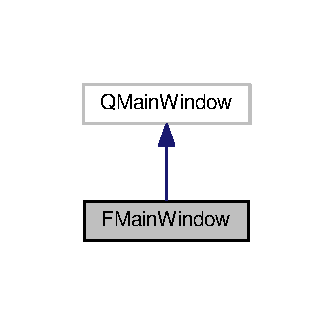
\includegraphics[width=160pt]{classFMainWindow__inherit__graph}
\end{center}
\end{figure}


Collaboration diagram for F\+Main\+Window\+:
\nopagebreak
\begin{figure}[H]
\begin{center}
\leavevmode
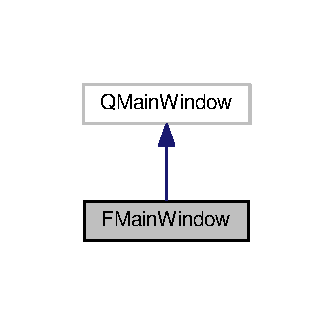
\includegraphics[width=160pt]{classFMainWindow__coll__graph}
\end{center}
\end{figure}
\subsection*{Signals}
\begin{DoxyCompactItemize}
\item 
\mbox{\Hypertarget{classFMainWindow_a42535d289ac70163aed4d818b2d5ea19}\label{classFMainWindow_a42535d289ac70163aed4d818b2d5ea19}} 
void {\bfseries signal\+\_\+open\+File\+Dialog} ()
\item 
\mbox{\Hypertarget{classFMainWindow_a27e577786cbea00f08362b46595b98e6}\label{classFMainWindow_a27e577786cbea00f08362b46595b98e6}} 
void {\bfseries signal\+\_\+show\+Help} ()
\item 
\mbox{\Hypertarget{classFMainWindow_a663f2f84ee547d310c01847b01c55bdc}\label{classFMainWindow_a663f2f84ee547d310c01847b01c55bdc}} 
void {\bfseries signal\+\_\+get\+Back} ()
\item 
\mbox{\Hypertarget{classFMainWindow_ae66529c44dc523c6d06a7961474868cf}\label{classFMainWindow_ae66529c44dc523c6d06a7961474868cf}} 
void {\bfseries load\+\_\+files} (const Q\+String\+List \&paths)
\item 
\mbox{\Hypertarget{classFMainWindow_aa80aa6dbaec6530ce381a2df4ba534c0}\label{classFMainWindow_aa80aa6dbaec6530ce381a2df4ba534c0}} 
void {\bfseries load\+\_\+files} (const Q\+List$<$ Q\+Url $>$ \&urls)
\end{DoxyCompactItemize}
\subsection*{Public Member Functions}
\begin{DoxyCompactItemize}
\item 
\mbox{\Hypertarget{classFMainWindow_a9ed1bc960f40fa9adec843a17df42d65}\label{classFMainWindow_a9ed1bc960f40fa9adec843a17df42d65}} 
{\bfseries F\+Main\+Window} (Q\+Widget $\ast$parent=0)
\end{DoxyCompactItemize}
\subsection*{Protected Slots}
\begin{DoxyCompactItemize}
\item 
\mbox{\Hypertarget{classFMainWindow_af565ef83f961c2dfeb6440aad2c74597}\label{classFMainWindow_af565ef83f961c2dfeb6440aad2c74597}} 
void {\bfseries open\+\_\+files} ()
\item 
\mbox{\Hypertarget{classFMainWindow_a45c72bba830f8cd2e2f6770b7e01fd3c}\label{classFMainWindow_a45c72bba830f8cd2e2f6770b7e01fd3c}} 
void {\bfseries show\+\_\+widget} ()
\item 
\mbox{\Hypertarget{classFMainWindow_af5889340ef407af53f6174ebd1d17d94}\label{classFMainWindow_af5889340ef407af53f6174ebd1d17d94}} 
void {\bfseries slot\+\_\+recognize\+\_\+webcam} ()
\end{DoxyCompactItemize}


The documentation for this class was generated from the following files\+:\begin{DoxyCompactItemize}
\item 
Facecope/widgets/include/\hyperlink{FMainWindow_8h}{F\+Main\+Window.\+h}\item 
Facecope/widgets/F\+Main\+Window.\+cpp\end{DoxyCompactItemize}

\hypertarget{classFSetFaceInfoDialog}{}\section{F\+Set\+Face\+Info\+Dialog Class Reference}
\label{classFSetFaceInfoDialog}\index{F\+Set\+Face\+Info\+Dialog@{F\+Set\+Face\+Info\+Dialog}}


Inheritance diagram for F\+Set\+Face\+Info\+Dialog\+:
\nopagebreak
\begin{figure}[H]
\begin{center}
\leavevmode
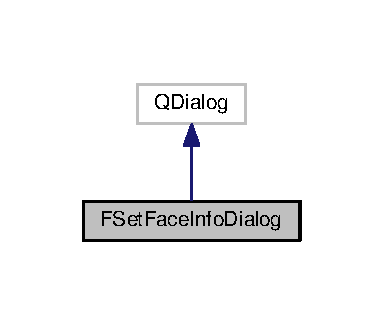
\includegraphics[width=184pt]{classFSetFaceInfoDialog__inherit__graph}
\end{center}
\end{figure}


Collaboration diagram for F\+Set\+Face\+Info\+Dialog\+:
\nopagebreak
\begin{figure}[H]
\begin{center}
\leavevmode
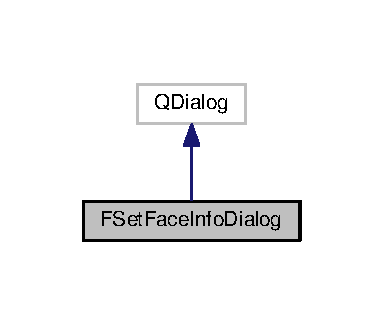
\includegraphics[width=184pt]{classFSetFaceInfoDialog__coll__graph}
\end{center}
\end{figure}
\subsection*{Public Member Functions}
\begin{DoxyCompactItemize}
\item 
\mbox{\Hypertarget{classFSetFaceInfoDialog_abbab58f313b3091cfd917b53f1590e9e}\label{classFSetFaceInfoDialog_abbab58f313b3091cfd917b53f1590e9e}} 
{\bfseries F\+Set\+Face\+Info\+Dialog} (\hyperlink{structFacecope}{Facecope} \&facecope, \hyperlink{classFFace}{F\+Face} \&face, \hyperlink{classFImage}{F\+Image} \&f\+\_\+image, Q\+Widget $\ast$parent=0)
\end{DoxyCompactItemize}


The documentation for this class was generated from the following files\+:\begin{DoxyCompactItemize}
\item 
Facecope/widgets/include/\hyperlink{FSetFaceInfoDialog_8h}{F\+Set\+Face\+Info\+Dialog.\+h}\item 
Facecope/widgets/F\+Set\+Face\+Info\+Dialog.\+cpp\end{DoxyCompactItemize}

\hypertarget{classFSettingsWidget}{}\section{F\+Settings\+Widget Class Reference}
\label{classFSettingsWidget}\index{F\+Settings\+Widget@{F\+Settings\+Widget}}


Inheritance diagram for F\+Settings\+Widget\+:
\nopagebreak
\begin{figure}[H]
\begin{center}
\leavevmode
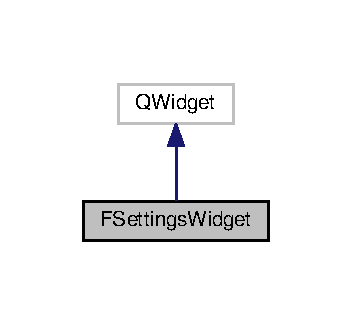
\includegraphics[width=169pt]{classFSettingsWidget__inherit__graph}
\end{center}
\end{figure}


Collaboration diagram for F\+Settings\+Widget\+:
\nopagebreak
\begin{figure}[H]
\begin{center}
\leavevmode
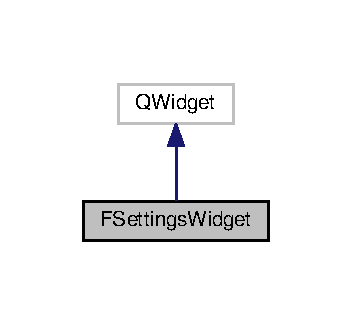
\includegraphics[width=169pt]{classFSettingsWidget__coll__graph}
\end{center}
\end{figure}
\subsection*{Public Member Functions}
\begin{DoxyCompactItemize}
\item 
\mbox{\Hypertarget{classFSettingsWidget_ae1b1d529212ec2bb4f05a941d86dc9a6}\label{classFSettingsWidget_ae1b1d529212ec2bb4f05a941d86dc9a6}} 
{\bfseries F\+Settings\+Widget} (\hyperlink{classSettings}{Settings} \&settings, Q\+Widget $\ast$parent=0)
\end{DoxyCompactItemize}


The documentation for this class was generated from the following files\+:\begin{DoxyCompactItemize}
\item 
Facecope/widgets/include/\hyperlink{FSettingsWidget_8h}{F\+Settings\+Widget.\+h}\item 
Facecope/widgets/F\+Settings\+Widget.\+cpp\end{DoxyCompactItemize}

\hypertarget{classFWorkingWidget}{}\section{F\+Working\+Widget Class Reference}
\label{classFWorkingWidget}\index{F\+Working\+Widget@{F\+Working\+Widget}}


Inheritance diagram for F\+Working\+Widget\+:
\nopagebreak
\begin{figure}[H]
\begin{center}
\leavevmode
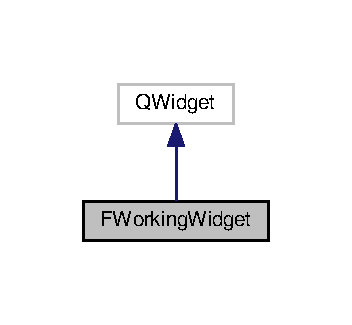
\includegraphics[width=169pt]{classFWorkingWidget__inherit__graph}
\end{center}
\end{figure}


Collaboration diagram for F\+Working\+Widget\+:
\nopagebreak
\begin{figure}[H]
\begin{center}
\leavevmode
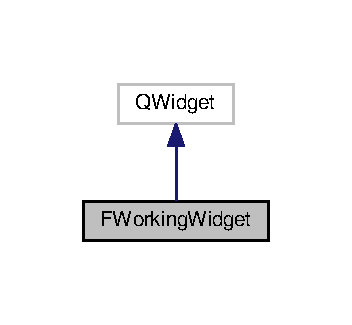
\includegraphics[width=169pt]{classFWorkingWidget__coll__graph}
\end{center}
\end{figure}
\subsection*{Public Slots}
\begin{DoxyCompactItemize}
\item 
\mbox{\Hypertarget{classFWorkingWidget_ada5c7a339541c0539af7b8c7404a4d1b}\label{classFWorkingWidget_ada5c7a339541c0539af7b8c7404a4d1b}} 
void {\bfseries slot\+\_\+add\+\_\+images} (const Q\+String\+List \&urls)
\item 
\mbox{\Hypertarget{classFWorkingWidget_abb592c30f0c97ecd92f82e98c0aa5328}\label{classFWorkingWidget_abb592c30f0c97ecd92f82e98c0aa5328}} 
void {\bfseries slot\+\_\+add\+\_\+images} (const Q\+List$<$ Q\+Url $>$ \&urls)
\item 
\mbox{\Hypertarget{classFWorkingWidget_a38c51fab9a4148a4250721973edd3f76}\label{classFWorkingWidget_a38c51fab9a4148a4250721973edd3f76}} 
void {\bfseries slot\+\_\+remove\+\_\+selected} ()
\item 
\mbox{\Hypertarget{classFWorkingWidget_a0b16dfaa4c53c5d92d0df10271784d2e}\label{classFWorkingWidget_a0b16dfaa4c53c5d92d0df10271784d2e}} 
void {\bfseries slot\+\_\+update\+\_\+labels} ()
\end{DoxyCompactItemize}
\subsection*{Signals}
\begin{DoxyCompactItemize}
\item 
\mbox{\Hypertarget{classFWorkingWidget_ac38f7d72616fcf31139f68f960cc67bc}\label{classFWorkingWidget_ac38f7d72616fcf31139f68f960cc67bc}} 
void {\bfseries signal\+\_\+update\+Item} (const Q\+String \&path)
\item 
\mbox{\Hypertarget{classFWorkingWidget_a84f5aa0893ce0ee469dfafa7760c2342}\label{classFWorkingWidget_a84f5aa0893ce0ee469dfafa7760c2342}} 
void {\bfseries signal\+\_\+images\+\_\+changed} ()
\item 
\mbox{\Hypertarget{classFWorkingWidget_a1a422682a4089845e7bbd2b8a44ba17d}\label{classFWorkingWidget_a1a422682a4089845e7bbd2b8a44ba17d}} 
void {\bfseries signal\+\_\+load\+\_\+images} (const Q\+List$<$ Q\+Url $>$ \&urls)
\item 
\mbox{\Hypertarget{classFWorkingWidget_ae501f074b45a1c9d98a827e1c92de889}\label{classFWorkingWidget_ae501f074b45a1c9d98a827e1c92de889}} 
void {\bfseries signal\+\_\+load\+\_\+images} (const Q\+String\+List \&urls)
\item 
\mbox{\Hypertarget{classFWorkingWidget_a249999260ac8e05d3eb0c3af10905566}\label{classFWorkingWidget_a249999260ac8e05d3eb0c3af10905566}} 
void {\bfseries signal\+\_\+detect\+\_\+face} (int row)
\end{DoxyCompactItemize}
\subsection*{Public Member Functions}
\begin{DoxyCompactItemize}
\item 
\mbox{\Hypertarget{classFWorkingWidget_a288d354166017dc56788e63c6fe1f97f}\label{classFWorkingWidget_a288d354166017dc56788e63c6fe1f97f}} 
{\bfseries F\+Working\+Widget} (\hyperlink{structFacecope}{Facecope} \&facecope, \hyperlink{classFMainFacecopeModel}{F\+Main\+Facecope\+Model} $\ast$model, Q\+Widget $\ast$parent=0)
\end{DoxyCompactItemize}


The documentation for this class was generated from the following files\+:\begin{DoxyCompactItemize}
\item 
Facecope/widgets/include/\hyperlink{FWorkingWidget_8h}{F\+Working\+Widget.\+h}\item 
Facecope/widgets/F\+Working\+Widget.\+cpp\end{DoxyCompactItemize}

\hypertarget{structHuman}{}\section{Human Struct Reference}
\label{structHuman}\index{Human@{Human}}


Collaboration diagram for Human\+:
\nopagebreak
\begin{figure}[H]
\begin{center}
\leavevmode
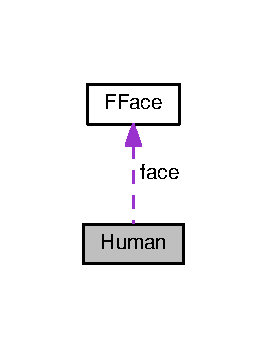
\includegraphics[width=128pt]{structHuman__coll__graph}
\end{center}
\end{figure}
\subsection*{Public Attributes}
\begin{DoxyCompactItemize}
\item 
\mbox{\Hypertarget{structHuman_a2f4d76356ea6ad90208b706a61228d1b}\label{structHuman_a2f4d76356ea6ad90208b706a61228d1b}} 
long {\bfseries ID}
\item 
\mbox{\Hypertarget{structHuman_a050c55e13eaf9b724e7cf83b12df7132}\label{structHuman_a050c55e13eaf9b724e7cf83b12df7132}} 
int {\bfseries gender}
\item 
\mbox{\Hypertarget{structHuman_a314b5ed988ef463a5479c5a864578367}\label{structHuman_a314b5ed988ef463a5479c5a864578367}} 
\hyperlink{classFFace}{F\+Face} $\ast$ {\bfseries face}
\item 
\mbox{\Hypertarget{structHuman_a97161abcfebe9461ef612f6cfde11e67}\label{structHuman_a97161abcfebe9461ef612f6cfde11e67}} 
Q\+String {\bfseries name}
\end{DoxyCompactItemize}


The documentation for this struct was generated from the following file\+:\begin{DoxyCompactItemize}
\item 
Facecope/\+Facecope\+Core/include/\hyperlink{FacecopeTypes_8h}{Facecope\+Types.\+h}\end{DoxyCompactItemize}

\hypertarget{classSettings}{}\section{Settings Class Reference}
\label{classSettings}\index{Settings@{Settings}}
\subsection*{Public Member Functions}
\begin{DoxyCompactItemize}
\item 
\mbox{\Hypertarget{classSettings_a4f2325e77317ffbfb532cce932b7ffa9}\label{classSettings_a4f2325e77317ffbfb532cce932b7ffa9}} 
Q\+String {\bfseries get\+Database\+\_\+path} () const
\item 
\mbox{\Hypertarget{classSettings_adcbf70b63bc3b1d0f86d5b97fb579ec8}\label{classSettings_adcbf70b63bc3b1d0f86d5b97fb579ec8}} 
Q\+String {\bfseries get\+Faces\+Prev\+\_\+path} () const
\item 
\mbox{\Hypertarget{classSettings_a66a13313a92a65f02ae991acfa73ff5a}\label{classSettings_a66a13313a92a65f02ae991acfa73ff5a}} 
Q\+String {\bfseries get\+Recognizer\+\_\+path} () const
\item 
\mbox{\Hypertarget{classSettings_a33a0681d2c594a22aa37becaa203d7dd}\label{classSettings_a33a0681d2c594a22aa37becaa203d7dd}} 
Q\+String {\bfseries get\+Recognizer\+\_\+gender\+\_\+path} () const
\item 
\mbox{\Hypertarget{classSettings_acc4435e11cd77355c867d58216432ffb}\label{classSettings_acc4435e11cd77355c867d58216432ffb}} 
Q\+String {\bfseries get\+Save\+\_\+settings\+\_\+path} () const
\item 
\mbox{\Hypertarget{classSettings_a6f12c7cbcca9bed562450d393db4f697}\label{classSettings_a6f12c7cbcca9bed562450d393db4f697}} 
void {\bfseries load} (const Q\+String \&path)
\item 
\mbox{\Hypertarget{classSettings_abd720f5e7a5eaea964578eab151da989}\label{classSettings_abd720f5e7a5eaea964578eab151da989}} 
void {\bfseries save} (const Q\+String \&path=Q\+String())
\item 
\mbox{\Hypertarget{classSettings_ad9bd331d9b049bf8d37cd94815c9dbfd}\label{classSettings_ad9bd331d9b049bf8d37cd94815c9dbfd}} 
void {\bfseries use\+Default} ()
\item 
\mbox{\Hypertarget{classSettings_abc0f51cf1d20d0023e940b343c8e68b0}\label{classSettings_abc0f51cf1d20d0023e940b343c8e68b0}} 
Q\+String {\bfseries get\+Output\+\_\+path} () const
\item 
\mbox{\Hypertarget{classSettings_aadff2d91d4479ccf743f3ae7510e2d20}\label{classSettings_aadff2d91d4479ccf743f3ae7510e2d20}} 
void {\bfseries set\+Output\+\_\+path} (const Q\+String \&output\+\_\+path)
\item 
\mbox{\Hypertarget{classSettings_a257b268ea7c9c498fb9d3235d01fac19}\label{classSettings_a257b268ea7c9c498fb9d3235d01fac19}} 
bool {\bfseries get\+Skip\+\_\+un\+Recognized} () const
\item 
\mbox{\Hypertarget{classSettings_a47af75ae812e9448e610ae3abef22fab}\label{classSettings_a47af75ae812e9448e610ae3abef22fab}} 
void {\bfseries set\+Skip\+\_\+un\+Recognized} (bool skip\+\_\+un\+Recognized)
\item 
\mbox{\Hypertarget{classSettings_a0c8d329d5c4894e5dd4aa5e2895e2c0e}\label{classSettings_a0c8d329d5c4894e5dd4aa5e2895e2c0e}} 
bool {\bfseries get\+Cut\+\_\+files} () const
\item 
\mbox{\Hypertarget{classSettings_af52bdf032abc5834eafdeee3c90bc4b1}\label{classSettings_af52bdf032abc5834eafdeee3c90bc4b1}} 
void {\bfseries set\+Cut\+\_\+files} (bool cut\+\_\+files)
\item 
\mbox{\Hypertarget{classSettings_a68e897fadeec6ca161e1ddd8474fd526}\label{classSettings_a68e897fadeec6ca161e1ddd8474fd526}} 
bool {\bfseries get\+Learn\+\_\+gender} () const
\item 
\mbox{\Hypertarget{classSettings_a5a7c4c75111a27069494338c37fc67ae}\label{classSettings_a5a7c4c75111a27069494338c37fc67ae}} 
void {\bfseries set\+Learn\+\_\+gender} (bool learn\+\_\+gender)
\item 
\mbox{\Hypertarget{classSettings_ac486fc156195d8ce64cd456d5b5d7bfb}\label{classSettings_ac486fc156195d8ce64cd456d5b5d7bfb}} 
bool {\bfseries get\+Learn\+\_\+recognized} () const
\item 
\mbox{\Hypertarget{classSettings_a79ae5d1bb99b8895574652f185348ffd}\label{classSettings_a79ae5d1bb99b8895574652f185348ffd}} 
void {\bfseries set\+Learn\+\_\+recognized} (bool learn\+\_\+recognized)
\item 
\mbox{\Hypertarget{classSettings_ae66c185fa4b028a2ead36d2a7c31fdcb}\label{classSettings_ae66c185fa4b028a2ead36d2a7c31fdcb}} 
int {\bfseries get\+Steps\+\_\+of\+\_\+detection} () const
\item 
\mbox{\Hypertarget{classSettings_a79a94f2ae969e79a788283d1c3c3139d}\label{classSettings_a79a94f2ae969e79a788283d1c3c3139d}} 
void {\bfseries set\+Steps\+\_\+of\+\_\+detection} (int steps\+\_\+of\+\_\+detection)
\item 
\mbox{\Hypertarget{classSettings_aa7ed74188185598a4cebc82f56e9789f}\label{classSettings_aa7ed74188185598a4cebc82f56e9789f}} 
int {\bfseries get\+Cascade\+\_\+type} () const
\item 
\mbox{\Hypertarget{classSettings_a78eae3234274546189cda1ed0a23474e}\label{classSettings_a78eae3234274546189cda1ed0a23474e}} 
void {\bfseries set\+Cascade\+\_\+type} (int cascade\+\_\+type)
\item 
\mbox{\Hypertarget{classSettings_abe7d3259a7f2716282fd836f0c098c71}\label{classSettings_abe7d3259a7f2716282fd836f0c098c71}} 
double {\bfseries get\+Threahold} () const
\item 
\mbox{\Hypertarget{classSettings_afac24f0d98c2ad0e7cefa606b069b3bb}\label{classSettings_afac24f0d98c2ad0e7cefa606b069b3bb}} 
void {\bfseries set\+Threahold} (double threahold)
\end{DoxyCompactItemize}


The documentation for this class was generated from the following files\+:\begin{DoxyCompactItemize}
\item 
Facecope/\+Facecope\+Core/include/Settings.\+h\item 
Facecope/\+Facecope\+Core/Settings.\+cpp\end{DoxyCompactItemize}

\chapter{File Documentation}
\hypertarget{FacecopeTypes_8h}{}\section{Facecope/\+Facecope\+Core/include/\+Facecope\+Types.h File Reference}
\label{FacecopeTypes_8h}\index{Facecope/\+Facecope\+Core/include/\+Facecope\+Types.\+h@{Facecope/\+Facecope\+Core/include/\+Facecope\+Types.\+h}}


defines core functional of \hyperlink{structFacecope}{Facecope}  


{\ttfamily \#include $<$Q\+String$>$}\newline
{\ttfamily \#include $<$opencv2/imgproc.\+hpp$>$}\newline
Include dependency graph for Facecope\+Types.\+h\+:
\nopagebreak
\begin{figure}[H]
\begin{center}
\leavevmode
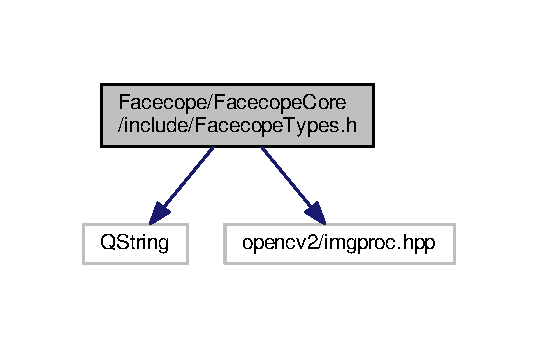
\includegraphics[width=258pt]{FacecopeTypes_8h__incl}
\end{center}
\end{figure}
This graph shows which files directly or indirectly include this file\+:
\nopagebreak
\begin{figure}[H]
\begin{center}
\leavevmode
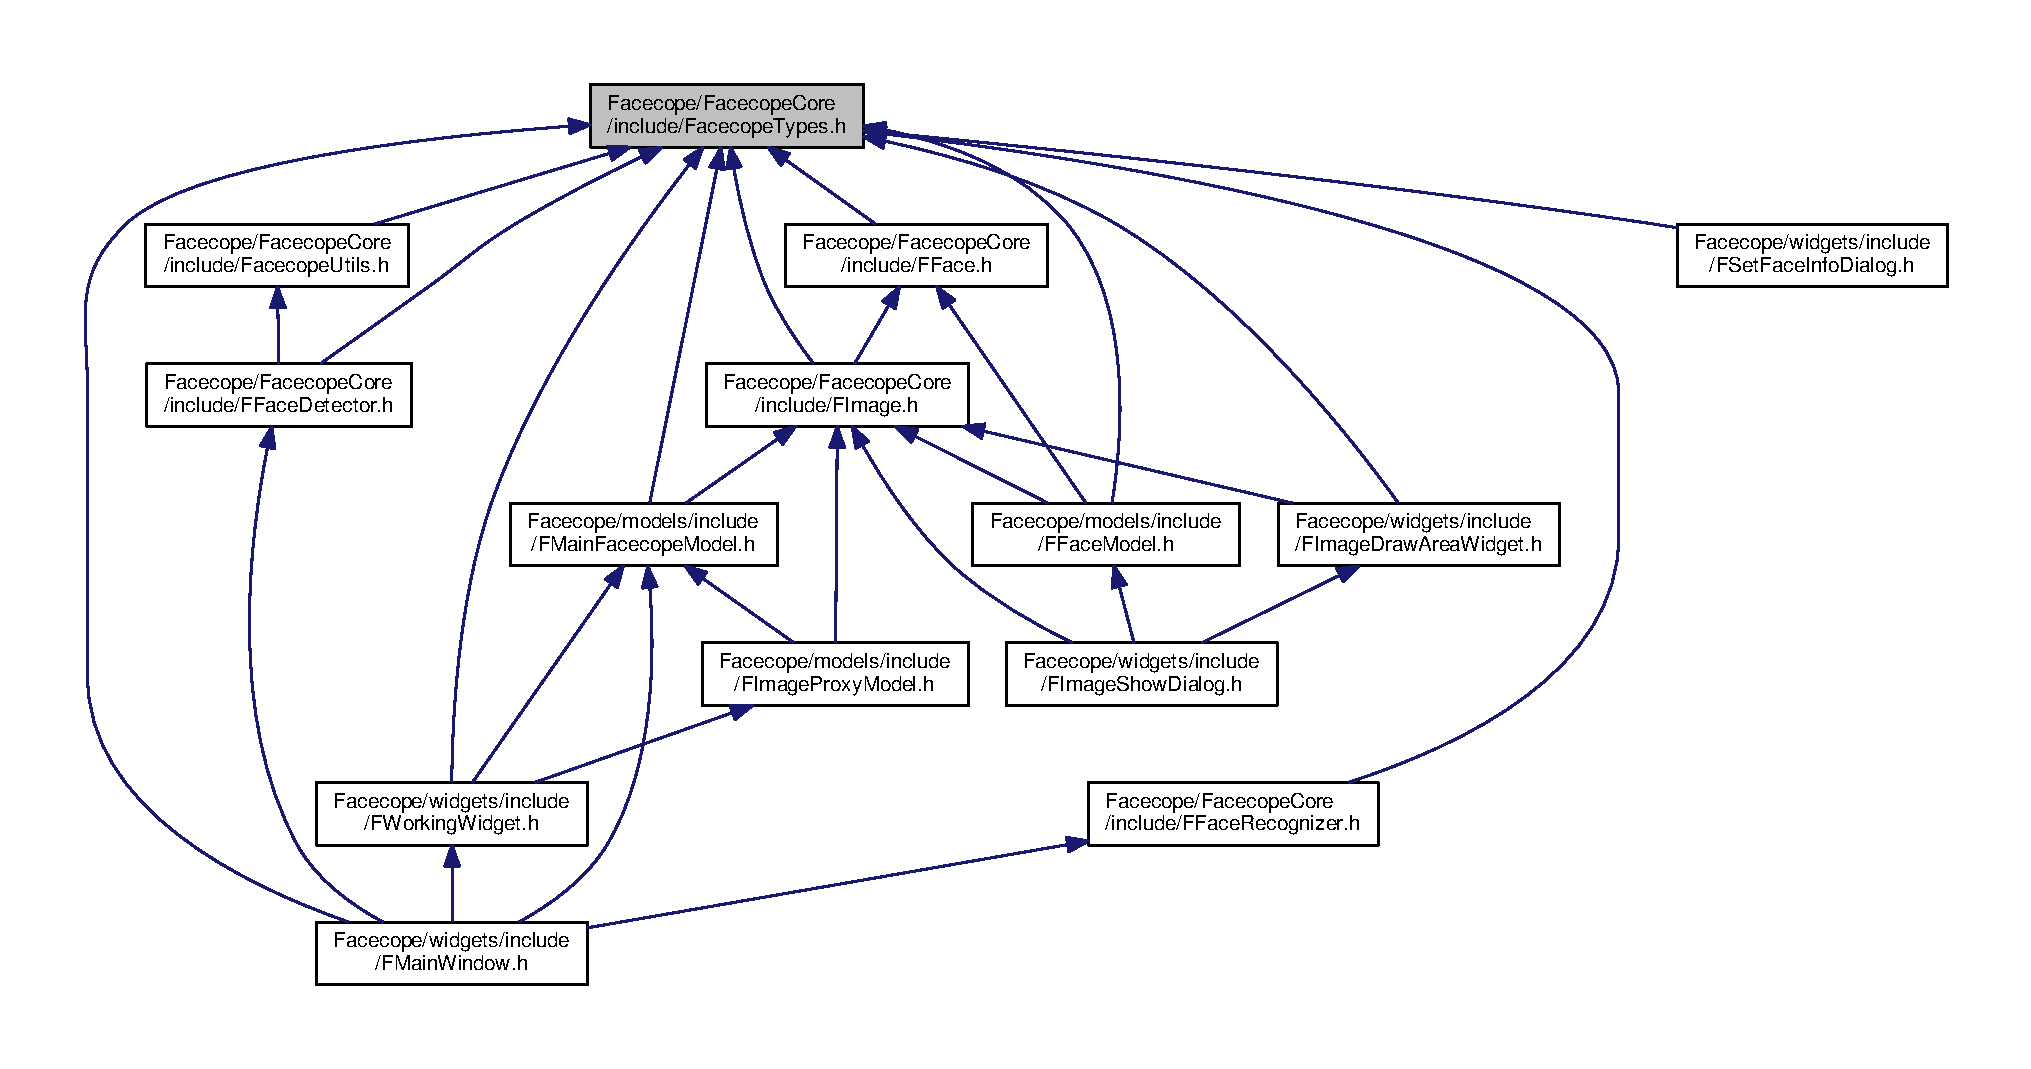
\includegraphics[width=350pt]{FacecopeTypes_8h__dep__incl}
\end{center}
\end{figure}
\subsection*{Classes}
\begin{DoxyCompactItemize}
\item 
struct \hyperlink{structEye}{Eye}
\item 
struct \hyperlink{structHuman}{Human}
\item 
struct \hyperlink{structFacecope}{Facecope}
\end{DoxyCompactItemize}
\subsection*{Enumerations}
\begin{DoxyCompactItemize}
\item 
\mbox{\Hypertarget{FacecopeTypes_8h_a06fc87d81c62e9abb8790b6e5713c55b}\label{FacecopeTypes_8h_a06fc87d81c62e9abb8790b6e5713c55b}} 
enum \{ {\bfseries M\+A\+LE} = 1, 
{\bfseries F\+E\+M\+A\+LE} = 2, 
{\bfseries U\+N\+R\+E\+C\+O\+G\+N\+I\+Z\+ED} = -\/1
 \}
\end{DoxyCompactItemize}
\subsection*{Functions}
\begin{DoxyCompactItemize}
\item 
\mbox{\Hypertarget{FacecopeTypes_8h_a3b66a85971e87d93214bc467f5856703}\label{FacecopeTypes_8h_a3b66a85971e87d93214bc467f5856703}} 
void {\bfseries learn\+New\+Human} (\hyperlink{structFacecope}{Facecope} \&facecope, int ID, int gender)
\end{DoxyCompactItemize}
\subsection*{Variables}
\begin{DoxyCompactItemize}
\item 
\mbox{\Hypertarget{FacecopeTypes_8h_a48450a9cbafdce38a37d95c6cbe5fee0}\label{FacecopeTypes_8h_a48450a9cbafdce38a37d95c6cbe5fee0}} 
enum  \{ ... \}  {\bfseries Sex}
\end{DoxyCompactItemize}


\subsection{Detailed Description}
defines core functional of \hyperlink{structFacecope}{Facecope} 


\hypertarget{FacecopeUtils_8h}{}\section{Facecope/\+Facecope\+Core/include/\+Facecope\+Utils.h File Reference}
\label{FacecopeUtils_8h}\index{Facecope/\+Facecope\+Core/include/\+Facecope\+Utils.\+h@{Facecope/\+Facecope\+Core/include/\+Facecope\+Utils.\+h}}


defines usefull fuctions for image transforation  


{\ttfamily \#include $<$Facecope\+Types.\+h$>$}\newline
{\ttfamily \#include $<$Q\+Image$>$}\newline
{\ttfamily \#include $<$Q\+String$>$}\newline
{\ttfamily \#include $<$opencv2/imgproc.\+hpp$>$}\newline
Include dependency graph for Facecope\+Utils.\+h\+:
\nopagebreak
\begin{figure}[H]
\begin{center}
\leavevmode
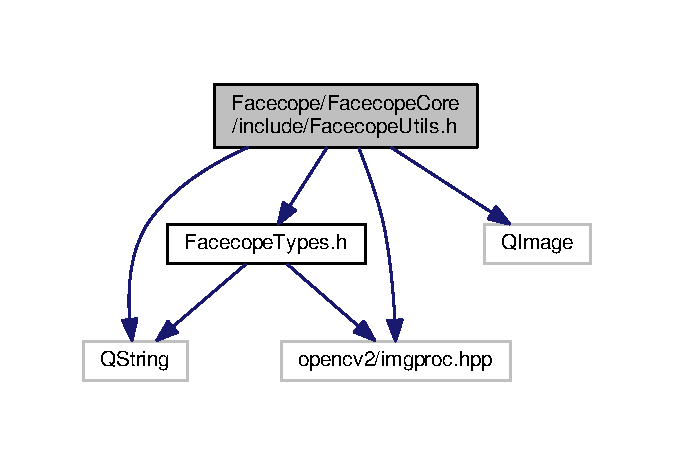
\includegraphics[width=324pt]{FacecopeUtils_8h__incl}
\end{center}
\end{figure}
This graph shows which files directly or indirectly include this file\+:
\nopagebreak
\begin{figure}[H]
\begin{center}
\leavevmode
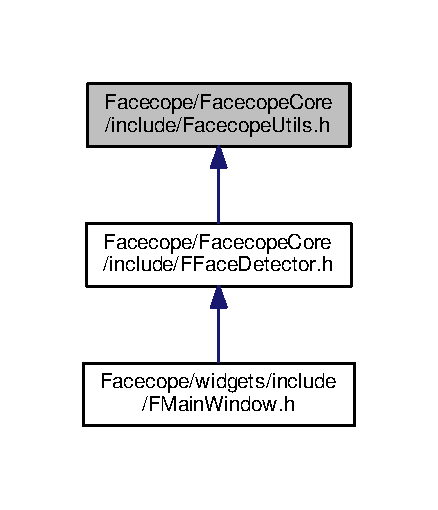
\includegraphics[width=210pt]{FacecopeUtils_8h__dep__incl}
\end{center}
\end{figure}
\subsection*{Functions}
\begin{DoxyCompactItemize}
\item 
\mbox{\Hypertarget{FacecopeUtils_8h_a6c96cc230a295d8c1fc9c9e27f73d7eb}\label{FacecopeUtils_8h_a6c96cc230a295d8c1fc9c9e27f73d7eb}} 
Q\+Image {\bfseries Mat2\+Q\+Image} (const cv\+::\+Mat \&cv\+\_\+image)
\item 
\mbox{\Hypertarget{FacecopeUtils_8h_a588fe30cf79103aba88c3558b4d34915}\label{FacecopeUtils_8h_a588fe30cf79103aba88c3558b4d34915}} 
cv\+::\+Mat {\bfseries Q\+Image2\+Mat} (const Q\+Image \&q\+\_\+image)
\item 
\mbox{\Hypertarget{FacecopeUtils_8h_abfe582409bcd7f0348692611f4d9b48b}\label{FacecopeUtils_8h_abfe582409bcd7f0348692611f4d9b48b}} 
bool {\bfseries is\+Image} (const Q\+String \&path)
\item 
\mbox{\Hypertarget{FacecopeUtils_8h_a42938b905cd2fc15914b4ad4c89519fe}\label{FacecopeUtils_8h_a42938b905cd2fc15914b4ad4c89519fe}} 
cv\+::\+Mat {\bfseries to\+Gray} (const cv\+::\+Mat \&src)
\item 
\mbox{\Hypertarget{FacecopeUtils_8h_a83fbeac8ca9be52ddcb69a0a03a1216d}\label{FacecopeUtils_8h_a83fbeac8ca9be52ddcb69a0a03a1216d}} 
cv\+::\+Mat {\bfseries cut} (const cv\+::\+Mat \&original, const cv\+::\+Rect \&frame)
\item 
\mbox{\Hypertarget{FacecopeUtils_8h_a8b6ec68f07e8687aa1924a8868cd5df0}\label{FacecopeUtils_8h_a8b6ec68f07e8687aa1924a8868cd5df0}} 
\hyperlink{structEye}{Eye} {\bfseries create\+Eye} (const cv\+::\+Rect \&frame)
\item 
\mbox{\Hypertarget{FacecopeUtils_8h_a7b743dba2e6894161831905c7752743f}\label{FacecopeUtils_8h_a7b743dba2e6894161831905c7752743f}} 
\hyperlink{structEye}{Eye} {\bfseries get\+Pair} (\hyperlink{structEye}{Eye} \&eye, const cv\+::\+Rect \&frame)
\item 
\mbox{\Hypertarget{FacecopeUtils_8h_aeacb9fcf0bd49a6530548454872fbae1}\label{FacecopeUtils_8h_aeacb9fcf0bd49a6530548454872fbae1}} 
cv\+::\+Point {\bfseries get\+Center} (const cv\+::\+Rect \&rect)
\item 
\mbox{\Hypertarget{FacecopeUtils_8h_ad50ba094e4ffcb058262d846b15a87b8}\label{FacecopeUtils_8h_ad50ba094e4ffcb058262d846b15a87b8}} 
cv\+::\+Point {\bfseries get\+Center} (const cv\+::\+Mat \&M)
\item 
\mbox{\Hypertarget{FacecopeUtils_8h_a07fbb220752489abc0f8f1c531739001}\label{FacecopeUtils_8h_a07fbb220752489abc0f8f1c531739001}} 
bool {\bfseries is\+File\+Exist} (const std\+::string \&path)
\item 
\mbox{\Hypertarget{FacecopeUtils_8h_abc260db414c3b757337994f9dc560737}\label{FacecopeUtils_8h_abc260db414c3b757337994f9dc560737}} 
float {\bfseries get\+Angle\+\_\+radians} (const cv\+::\+Point \&p1, const cv\+::\+Point \&p2)
\item 
\mbox{\Hypertarget{FacecopeUtils_8h_a46f4af3bc6187d57458df35b654b6df5}\label{FacecopeUtils_8h_a46f4af3bc6187d57458df35b654b6df5}} 
float {\bfseries to\+Degrees} (float radians)
\item 
\mbox{\Hypertarget{FacecopeUtils_8h_af2303ff3ec9c1d09c978fe6bcced33ee}\label{FacecopeUtils_8h_af2303ff3ec9c1d09c978fe6bcced33ee}} 
float {\bfseries to\+Radians} (float degree)
\item 
\mbox{\Hypertarget{FacecopeUtils_8h_a058d10b7bfade5dbfbf2c31cc985c34a}\label{FacecopeUtils_8h_a058d10b7bfade5dbfbf2c31cc985c34a}} 
cv\+::\+Size {\bfseries get\+Size} (const cv\+::\+Mat \&M, float scale)
\item 
\mbox{\Hypertarget{FacecopeUtils_8h_a8c064e59942fe91d03194f0d8702ddec}\label{FacecopeUtils_8h_a8c064e59942fe91d03194f0d8702ddec}} 
cv\+::\+Size {\bfseries get\+Size} (const cv\+::\+Rect \&R, float scale)
\item 
\mbox{\Hypertarget{FacecopeUtils_8h_adcd8eb6ae8250995106fd01ace424ee7}\label{FacecopeUtils_8h_adcd8eb6ae8250995106fd01ace424ee7}} 
void {\bfseries rotate\+Rect} (cv\+::\+Rect \&R, const cv\+::\+Point2f \&center, float angle)
\item 
\mbox{\Hypertarget{FacecopeUtils_8h_a6ec8a7cd0a66c0293f97ca9d7bbba7fe}\label{FacecopeUtils_8h_a6ec8a7cd0a66c0293f97ca9d7bbba7fe}} 
void {\bfseries rotate\+Point} (int \&x, int \&y, const cv\+::\+Point \&center, float angle)
\item 
\mbox{\Hypertarget{FacecopeUtils_8h_a9b33abe1c7579f7097105a6571ff63ee}\label{FacecopeUtils_8h_a9b33abe1c7579f7097105a6571ff63ee}} 
void {\bfseries rotate\+Point} (cv\+::\+Point \&point, const cv\+::\+Point \&center, float angle)
\item 
\mbox{\Hypertarget{FacecopeUtils_8h_a6346d71220bbdc2c11abc7b72602e76f}\label{FacecopeUtils_8h_a6346d71220bbdc2c11abc7b72602e76f}} 
cv\+::\+Mat {\bfseries rotate} (const cv\+::\+Mat \&image, float degree, bool increase\+Bounds=false)
\item 
\mbox{\Hypertarget{FacecopeUtils_8h_af3e733e53f31a385d86e8eb532e1ae7c}\label{FacecopeUtils_8h_af3e733e53f31a385d86e8eb532e1ae7c}} 
void {\bfseries disable\+Area} (cv\+::\+Mat \&image, const cv\+::\+Rect \&rect)
\end{DoxyCompactItemize}


\subsection{Detailed Description}
defines usefull fuctions for image transforation 


\hypertarget{FDatabaseDriver_8h}{}\section{Facecope/\+Facecope\+Core/include/\+F\+Database\+Driver.h File Reference}
\label{FDatabaseDriver_8h}\index{Facecope/\+Facecope\+Core/include/\+F\+Database\+Driver.\+h@{Facecope/\+Facecope\+Core/include/\+F\+Database\+Driver.\+h}}


defines database drivers, for work with facecope\textquotesingle{}s database  


{\ttfamily \#include $<$Q\+Map$>$}\newline
{\ttfamily \#include $<$Q\+Sql\+Driver$>$}\newline
{\ttfamily \#include $<$Q\+Sql\+Driver\+Creator\+Base$>$}\newline
{\ttfamily \#include $<$Q\+Sql\+Error$>$}\newline
{\ttfamily \#include $<$Q\+String$>$}\newline
{\ttfamily \#include $<$Settings.\+h$>$}\newline
Include dependency graph for F\+Database\+Driver.\+h\+:
\nopagebreak
\begin{figure}[H]
\begin{center}
\leavevmode
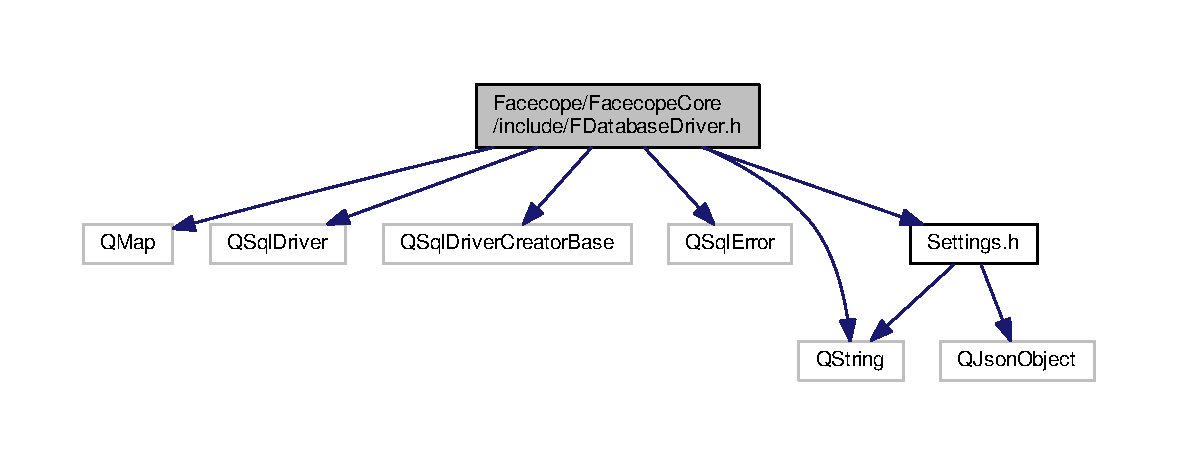
\includegraphics[width=350pt]{FDatabaseDriver_8h__incl}
\end{center}
\end{figure}
This graph shows which files directly or indirectly include this file\+:
\nopagebreak
\begin{figure}[H]
\begin{center}
\leavevmode
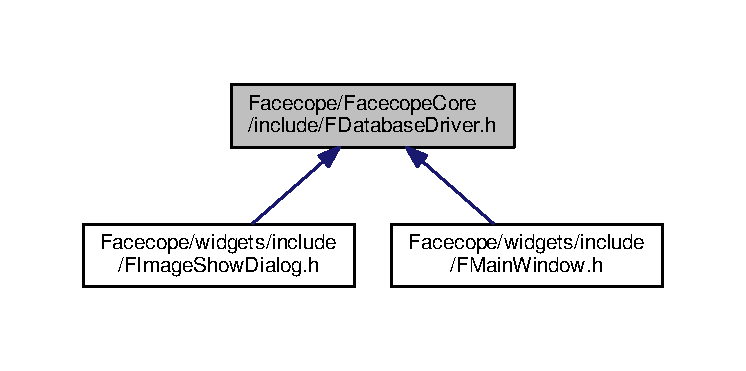
\includegraphics[width=350pt]{FDatabaseDriver_8h__dep__incl}
\end{center}
\end{figure}
\subsection*{Classes}
\begin{DoxyCompactItemize}
\item 
class \hyperlink{classFDatabaseDriver}{F\+Database\+Driver}
\end{DoxyCompactItemize}


\subsection{Detailed Description}
defines database drivers, for work with facecope\textquotesingle{}s database 


\hypertarget{FImage_8h}{}\section{Facecope/\+Facecope\+Core/include/\+F\+Image.h File Reference}
\label{FImage_8h}\index{Facecope/\+Facecope\+Core/include/\+F\+Image.\+h@{Facecope/\+Facecope\+Core/include/\+F\+Image.\+h}}


Declaration of the class of image storage and persons on it.  


{\ttfamily \#include $<$F\+Face.\+h$>$}\newline
{\ttfamily \#include $<$Facecope\+Types.\+h$>$}\newline
{\ttfamily \#include $<$Q\+Image$>$}\newline
{\ttfamily \#include $<$Q\+String$>$}\newline
{\ttfamily \#include $<$Q\+Vector$>$}\newline
{\ttfamily \#include $<$opencv2/imgproc.\+hpp$>$}\newline
{\ttfamily \#include $<$vector$>$}\newline
Include dependency graph for F\+Image.\+h\+:
\nopagebreak
\begin{figure}[H]
\begin{center}
\leavevmode
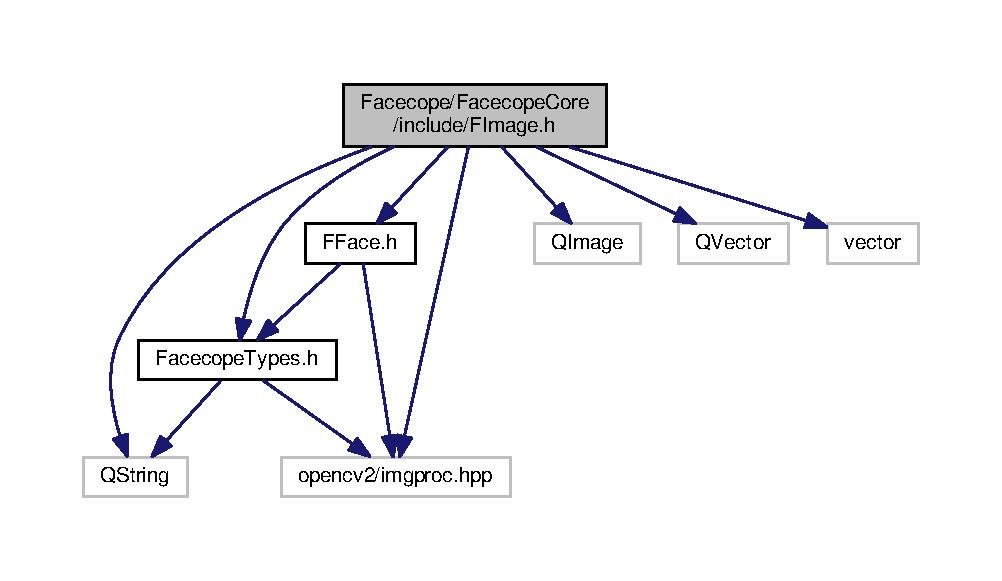
\includegraphics[width=350pt]{FImage_8h__incl}
\end{center}
\end{figure}
This graph shows which files directly or indirectly include this file\+:
\nopagebreak
\begin{figure}[H]
\begin{center}
\leavevmode
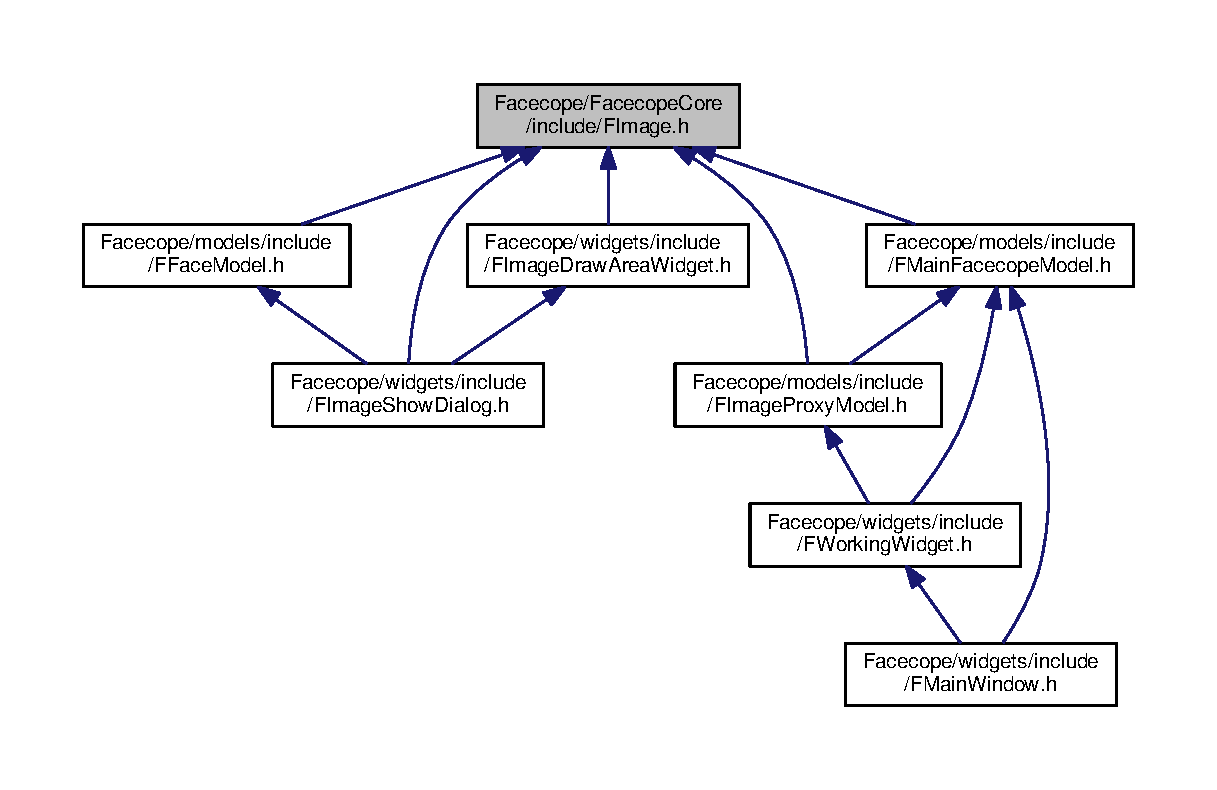
\includegraphics[width=350pt]{FImage_8h__dep__incl}
\end{center}
\end{figure}
\subsection*{Classes}
\begin{DoxyCompactItemize}
\item 
class \hyperlink{classFImage}{F\+Image}
\end{DoxyCompactItemize}


\subsection{Detailed Description}
Declaration of the class of image storage and persons on it. 


\hypertarget{FImageProxyModel_8h}{}\section{Facecope/models/include/\+F\+Image\+Proxy\+Model.h File Reference}
\label{FImageProxyModel_8h}\index{Facecope/models/include/\+F\+Image\+Proxy\+Model.\+h@{Facecope/models/include/\+F\+Image\+Proxy\+Model.\+h}}


Declaration of the class for image view filtering.  


{\ttfamily \#include $<$F\+Image.\+h$>$}\newline
{\ttfamily \#include $<$F\+Main\+Facecope\+Model.\+h$>$}\newline
{\ttfamily \#include $<$Q\+Set$>$}\newline
{\ttfamily \#include $<$Q\+Sort\+Filter\+Proxy\+Model$>$}\newline
Include dependency graph for F\+Image\+Proxy\+Model.\+h\+:
\nopagebreak
\begin{figure}[H]
\begin{center}
\leavevmode
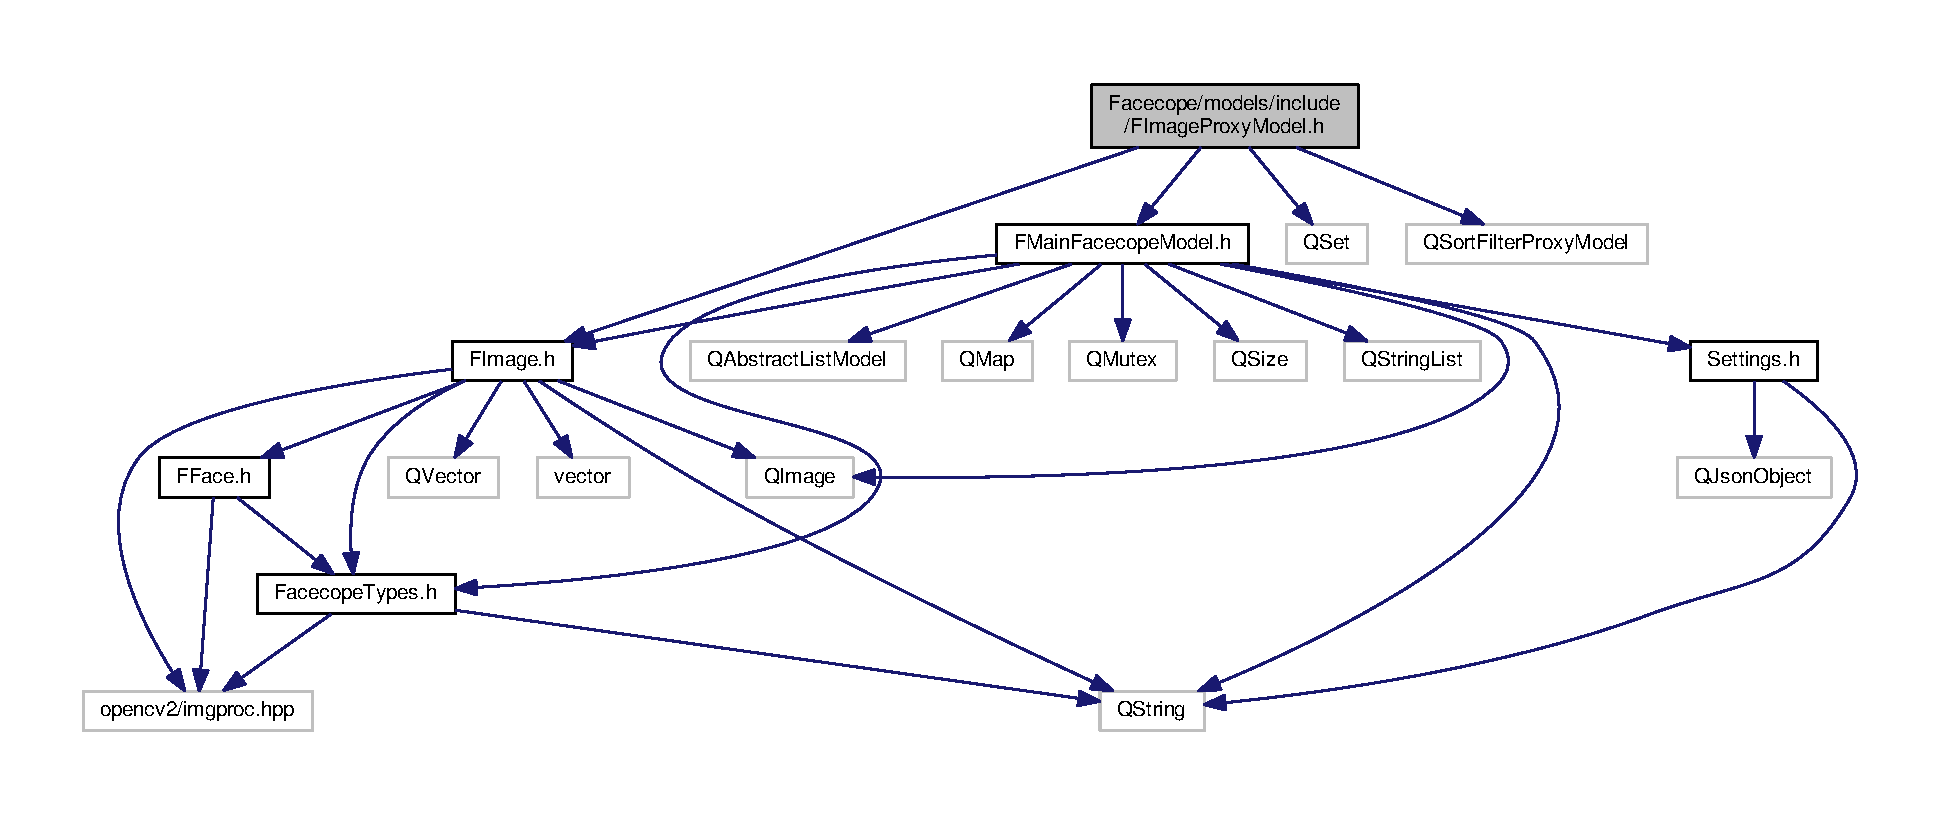
\includegraphics[width=350pt]{FImageProxyModel_8h__incl}
\end{center}
\end{figure}
This graph shows which files directly or indirectly include this file\+:
\nopagebreak
\begin{figure}[H]
\begin{center}
\leavevmode
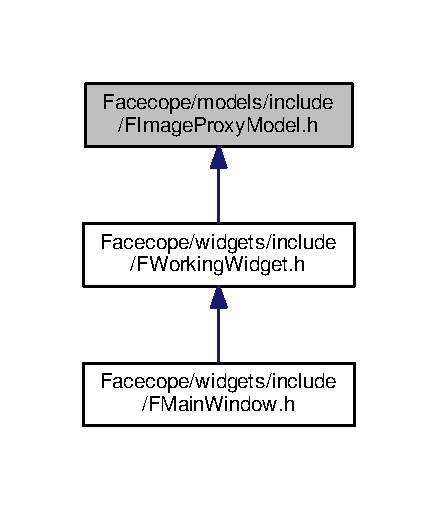
\includegraphics[width=210pt]{FImageProxyModel_8h__dep__incl}
\end{center}
\end{figure}
\subsection*{Classes}
\begin{DoxyCompactItemize}
\item 
class \hyperlink{classFImageProxyModel}{F\+Image\+Proxy\+Model}
\end{DoxyCompactItemize}


\subsection{Detailed Description}
Declaration of the class for image view filtering. 


\hypertarget{FMainFacecopeModel_8h}{}\section{Facecope/models/include/\+F\+Main\+Facecope\+Model.h File Reference}
\label{FMainFacecopeModel_8h}\index{Facecope/models/include/\+F\+Main\+Facecope\+Model.\+h@{Facecope/models/include/\+F\+Main\+Facecope\+Model.\+h}}


The announcement of the main model of user interaction with photo data.  


{\ttfamily \#include $<$F\+Image.\+h$>$}\newline
{\ttfamily \#include $<$Facecope\+Types.\+h$>$}\newline
{\ttfamily \#include $<$Q\+Abstract\+List\+Model$>$}\newline
{\ttfamily \#include $<$Q\+Image$>$}\newline
{\ttfamily \#include $<$Q\+Map$>$}\newline
{\ttfamily \#include $<$Q\+Mutex$>$}\newline
{\ttfamily \#include $<$Q\+Size$>$}\newline
{\ttfamily \#include $<$Q\+String$>$}\newline
{\ttfamily \#include $<$Settings.\+h$>$}\newline
{\ttfamily \#include $<$Q\+String\+List$>$}\newline
Include dependency graph for F\+Main\+Facecope\+Model.\+h\+:
\nopagebreak
\begin{figure}[H]
\begin{center}
\leavevmode
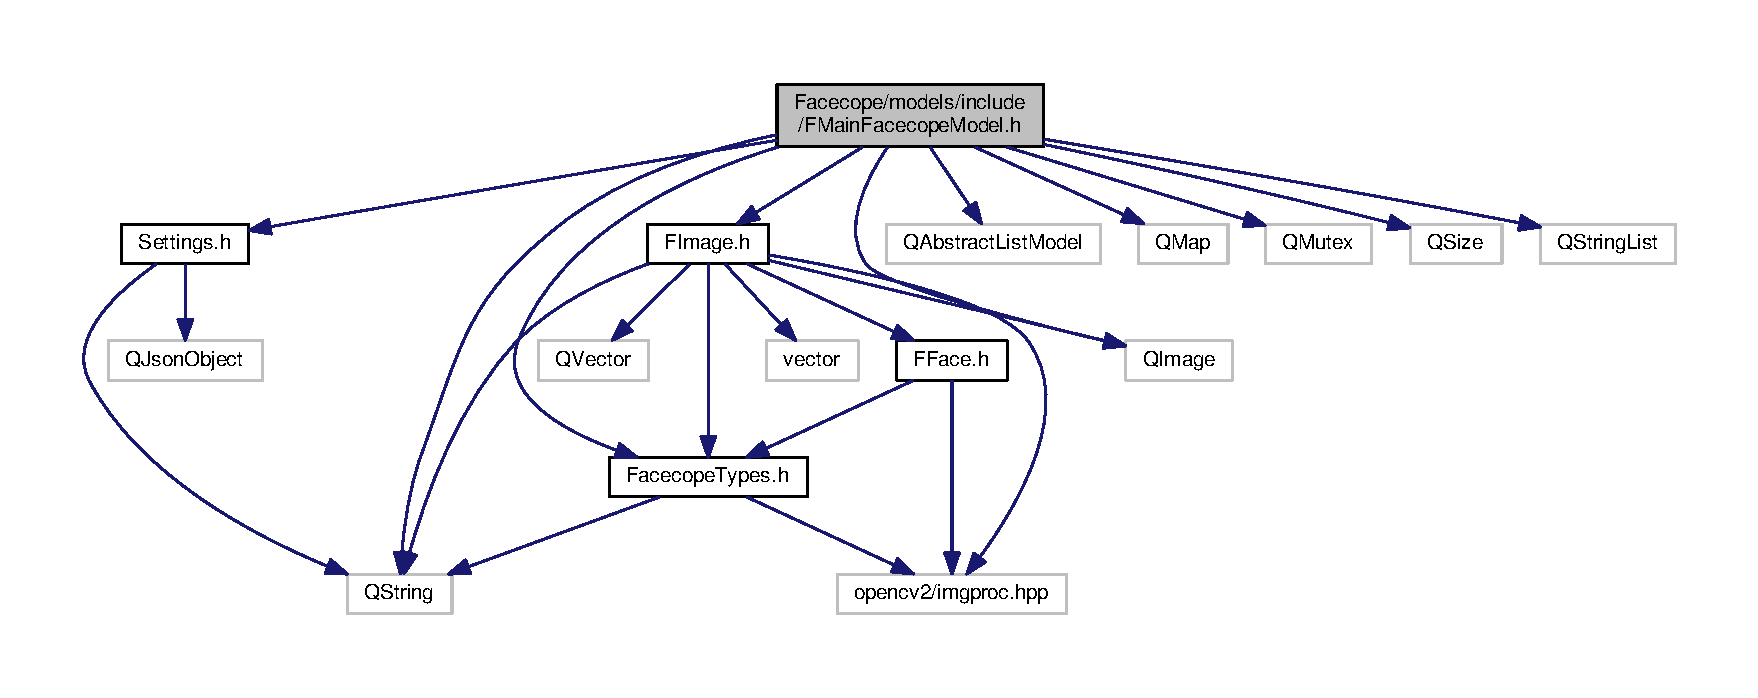
\includegraphics[width=350pt]{FMainFacecopeModel_8h__incl}
\end{center}
\end{figure}
This graph shows which files directly or indirectly include this file\+:
\nopagebreak
\begin{figure}[H]
\begin{center}
\leavevmode
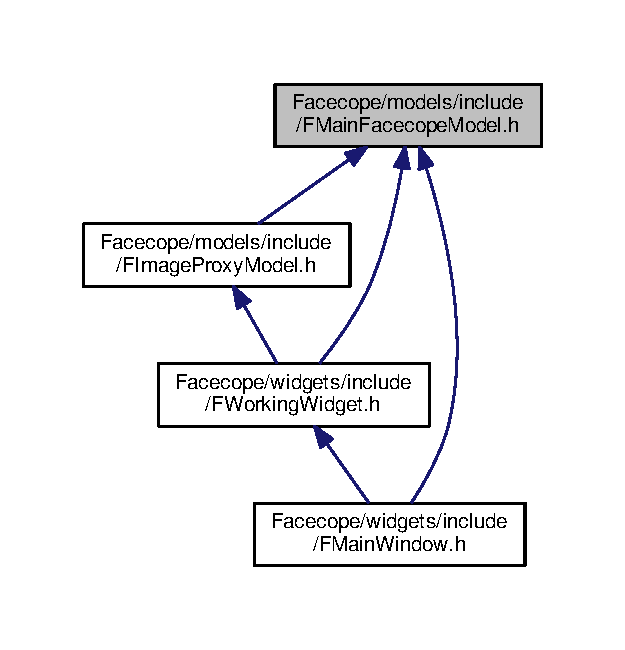
\includegraphics[width=300pt]{FMainFacecopeModel_8h__dep__incl}
\end{center}
\end{figure}
\subsection*{Classes}
\begin{DoxyCompactItemize}
\item 
class \hyperlink{classFMainFacecopeModel}{F\+Main\+Facecope\+Model}
\end{DoxyCompactItemize}
\subsection*{Enumerations}
\begin{DoxyCompactItemize}
\item 
\mbox{\Hypertarget{FMainFacecopeModel_8h_abc6126af1d45847bc59afa0aa3216b04}\label{FMainFacecopeModel_8h_abc6126af1d45847bc59afa0aa3216b04}} 
enum \{ {\bfseries G\+E\+T\+\_\+\+F\+U\+L\+L\+\_\+\+I\+T\+E\+M\+\_\+\+P\+A\+TH} = -\/1
 \}
\end{DoxyCompactItemize}


\subsection{Detailed Description}
The announcement of the main model of user interaction with photo data. 


\hypertarget{FHelpWidget_8h}{}\section{Facecope/widgets/include/\+F\+Help\+Widget.h File Reference}
\label{FHelpWidget_8h}\index{Facecope/widgets/include/\+F\+Help\+Widget.\+h@{Facecope/widgets/include/\+F\+Help\+Widget.\+h}}


defines help-\/widget  


{\ttfamily \#include $<$Q\+Widget$>$}\newline
Include dependency graph for F\+Help\+Widget.\+h\+:
\nopagebreak
\begin{figure}[H]
\begin{center}
\leavevmode
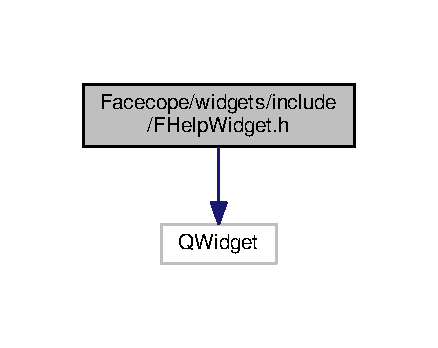
\includegraphics[width=210pt]{FHelpWidget_8h__incl}
\end{center}
\end{figure}
\subsection*{Classes}
\begin{DoxyCompactItemize}
\item 
class \hyperlink{classFHelpWidget}{F\+Help\+Widget}
\end{DoxyCompactItemize}


\subsection{Detailed Description}
defines help-\/widget 


\hypertarget{FImageDrawAreaWidget_8h}{}\section{Facecope/widgets/include/\+F\+Image\+Draw\+Area\+Widget.h File Reference}
\label{FImageDrawAreaWidget_8h}\index{Facecope/widgets/include/\+F\+Image\+Draw\+Area\+Widget.\+h@{Facecope/widgets/include/\+F\+Image\+Draw\+Area\+Widget.\+h}}


defines drawing area with faces-\/widget  


{\ttfamily \#include $<$Facecope\+Types.\+h$>$}\newline
{\ttfamily \#include $<$Q\+Pen$>$}\newline
{\ttfamily \#include $<$Q\+Widget$>$}\newline
{\ttfamily \#include $<$F\+Image.\+h$>$}\newline
{\ttfamily \#include $<$Settings.\+h$>$}\newline
Include dependency graph for F\+Image\+Draw\+Area\+Widget.\+h\+:
\nopagebreak
\begin{figure}[H]
\begin{center}
\leavevmode
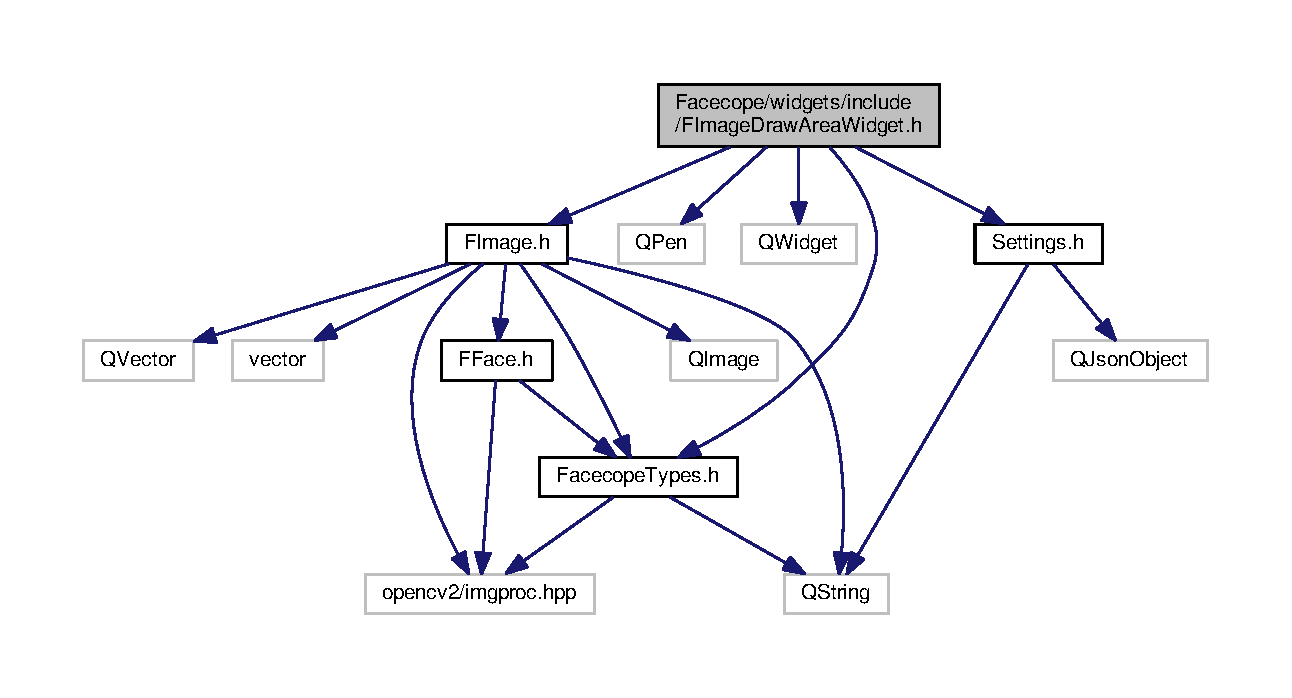
\includegraphics[width=350pt]{FImageDrawAreaWidget_8h__incl}
\end{center}
\end{figure}
This graph shows which files directly or indirectly include this file\+:
\nopagebreak
\begin{figure}[H]
\begin{center}
\leavevmode
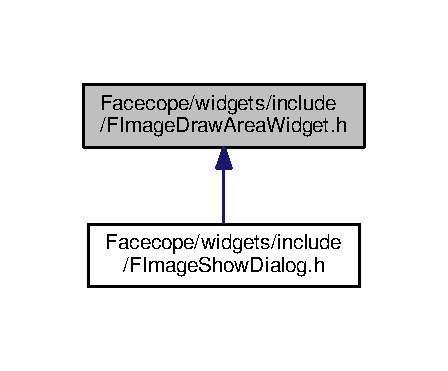
\includegraphics[width=215pt]{FImageDrawAreaWidget_8h__dep__incl}
\end{center}
\end{figure}
\subsection*{Classes}
\begin{DoxyCompactItemize}
\item 
class \hyperlink{classFImageDrawAreaWidget}{F\+Image\+Draw\+Area\+Widget}
\end{DoxyCompactItemize}


\subsection{Detailed Description}
defines drawing area with faces-\/widget 


\hypertarget{FImageShowDialog_8h}{}\section{Facecope/widgets/include/\+F\+Image\+Show\+Dialog.h File Reference}
\label{FImageShowDialog_8h}\index{Facecope/widgets/include/\+F\+Image\+Show\+Dialog.\+h@{Facecope/widgets/include/\+F\+Image\+Show\+Dialog.\+h}}


defines dialog for lavel viewing and editing  


{\ttfamily \#include $<$F\+Database\+Driver.\+h$>$}\newline
{\ttfamily \#include $<$F\+Face\+Model.\+h$>$}\newline
{\ttfamily \#include $<$F\+Image.\+h$>$}\newline
{\ttfamily \#include $<$F\+Image\+Draw\+Area\+Widget.\+h$>$}\newline
{\ttfamily \#include $<$Q\+Dialog$>$}\newline
{\ttfamily \#include $<$Settings.\+h$>$}\newline
Include dependency graph for F\+Image\+Show\+Dialog.\+h\+:
\nopagebreak
\begin{figure}[H]
\begin{center}
\leavevmode
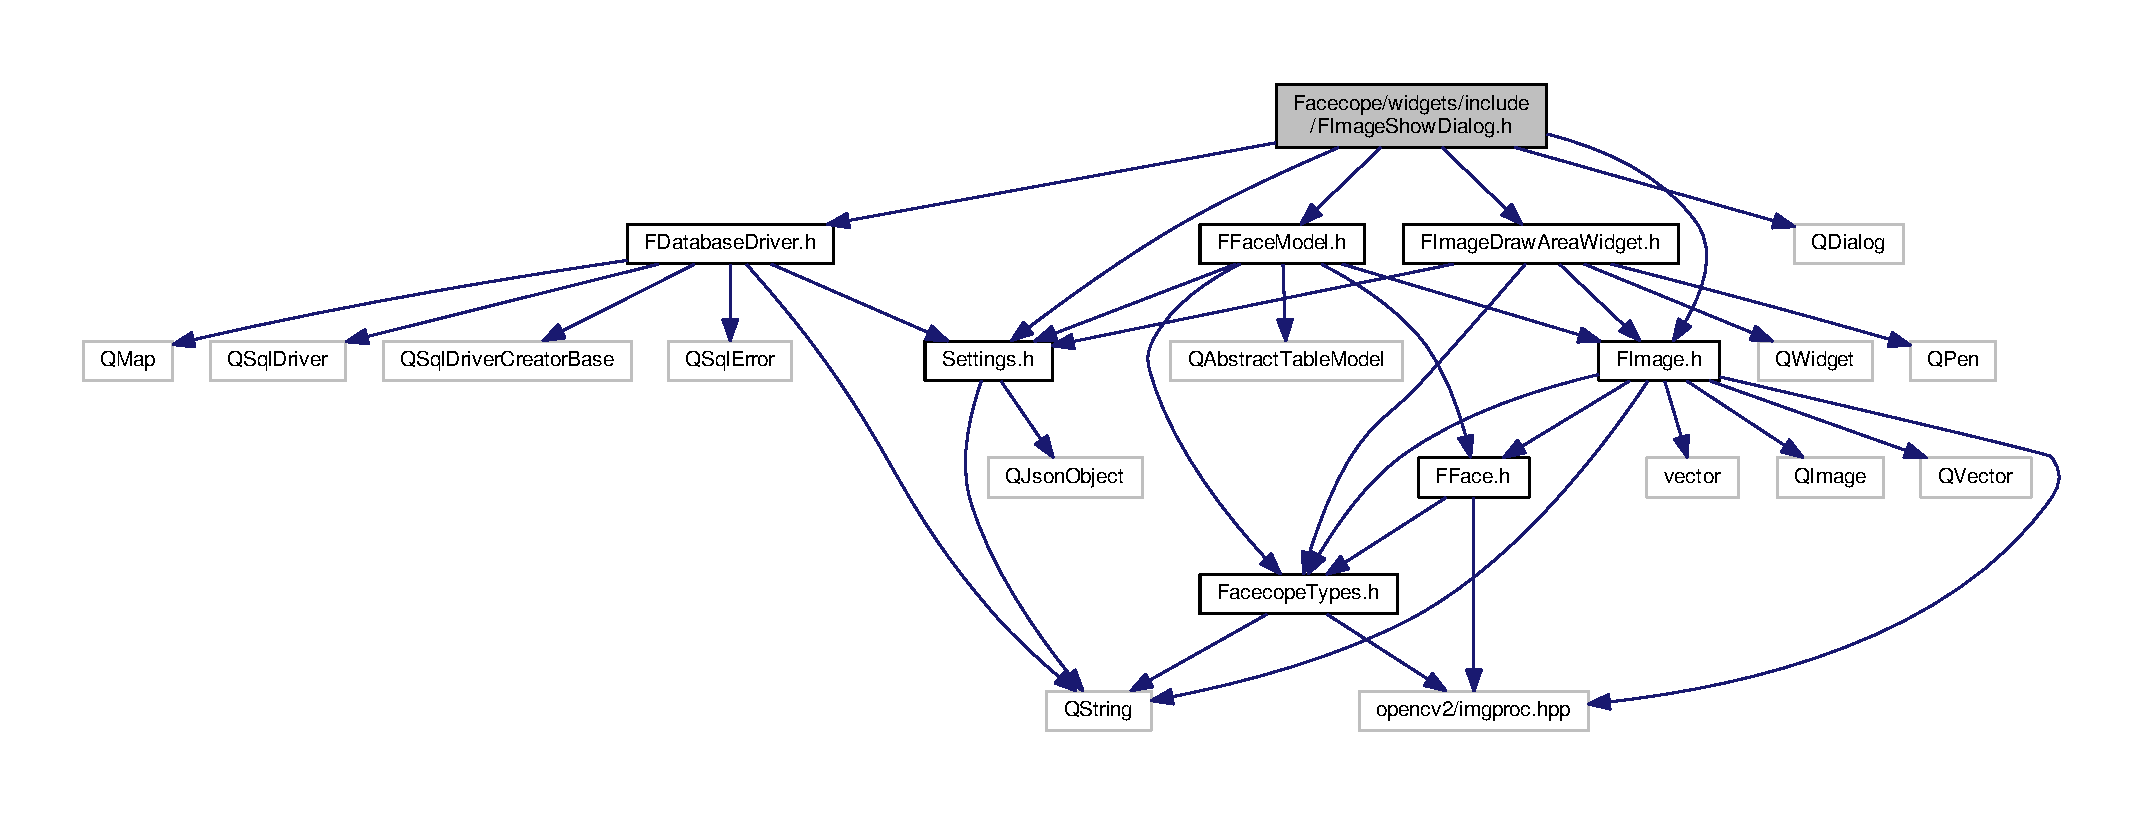
\includegraphics[width=350pt]{FImageShowDialog_8h__incl}
\end{center}
\end{figure}
\subsection*{Classes}
\begin{DoxyCompactItemize}
\item 
class \hyperlink{classFImageShowDialog}{F\+Image\+Show\+Dialog}
\end{DoxyCompactItemize}


\subsection{Detailed Description}
defines dialog for lavel viewing and editing 


\hypertarget{FMainWindow_8h}{}\section{Facecope/widgets/include/\+F\+Main\+Window.h File Reference}
\label{FMainWindow_8h}\index{Facecope/widgets/include/\+F\+Main\+Window.\+h@{Facecope/widgets/include/\+F\+Main\+Window.\+h}}


main container of widgets  


{\ttfamily \#include $<$F\+Database\+Driver.\+h$>$}\newline
{\ttfamily \#include $<$F\+Face\+Detector.\+h$>$}\newline
{\ttfamily \#include $<$F\+Face\+Recognizer.\+h$>$}\newline
{\ttfamily \#include $<$F\+Main\+Facecope\+Model.\+h$>$}\newline
{\ttfamily \#include $<$F\+Working\+Widget.\+h$>$}\newline
{\ttfamily \#include $<$Facecope\+Types.\+h$>$}\newline
{\ttfamily \#include $<$Q\+List$>$}\newline
{\ttfamily \#include $<$Q\+Main\+Window$>$}\newline
{\ttfamily \#include $<$Q\+Map$>$}\newline
{\ttfamily \#include $<$Q\+String\+List$>$}\newline
{\ttfamily \#include $<$Q\+Url$>$}\newline
{\ttfamily \#include $<$Settings.\+h$>$}\newline
Include dependency graph for F\+Main\+Window.\+h\+:
\nopagebreak
\begin{figure}[H]
\begin{center}
\leavevmode
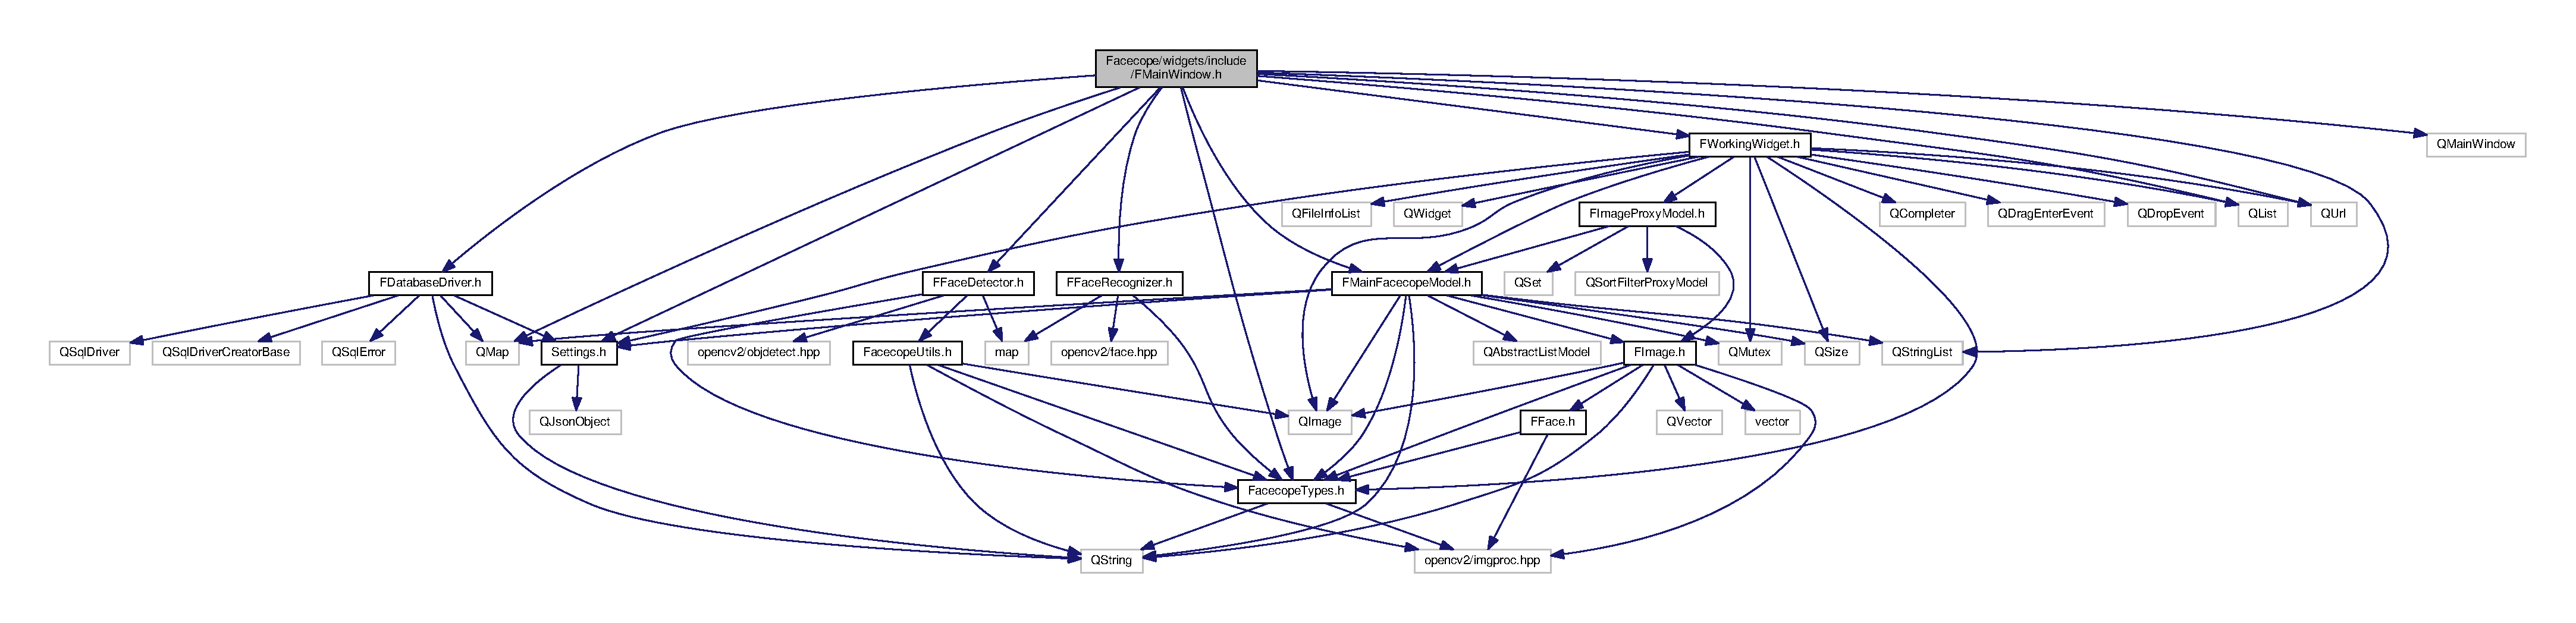
\includegraphics[width=350pt]{FMainWindow_8h__incl}
\end{center}
\end{figure}
\subsection*{Classes}
\begin{DoxyCompactItemize}
\item 
class \hyperlink{classFMainWindow}{F\+Main\+Window}
\end{DoxyCompactItemize}
\subsection*{Macros}
\begin{DoxyCompactItemize}
\item 
\mbox{\Hypertarget{FMainWindow_8h_afc1cfb5a0bf2af2664cccd67d53aa0b8}\label{FMainWindow_8h_afc1cfb5a0bf2af2664cccd67d53aa0b8}} 
\#define {\bfseries R\+E\+S\+O\+U\+R\+C\+E\+\_\+\+P\+A\+TH}~\char`\"{}../../res/\char`\"{}
\end{DoxyCompactItemize}


\subsection{Detailed Description}
main container of widgets 


\hypertarget{FSetFaceInfoDialog_8h}{}\section{Facecope/widgets/include/\+F\+Set\+Face\+Info\+Dialog.h File Reference}
\label{FSetFaceInfoDialog_8h}\index{Facecope/widgets/include/\+F\+Set\+Face\+Info\+Dialog.\+h@{Facecope/widgets/include/\+F\+Set\+Face\+Info\+Dialog.\+h}}


defines dialog for editing labels of face  


{\ttfamily \#include $<$Facecope\+Types.\+h$>$}\newline
{\ttfamily \#include $<$Q\+Dialog$>$}\newline
{\ttfamily \#include $<$Q\+Image$>$}\newline
Include dependency graph for F\+Set\+Face\+Info\+Dialog.\+h\+:
\nopagebreak
\begin{figure}[H]
\begin{center}
\leavevmode
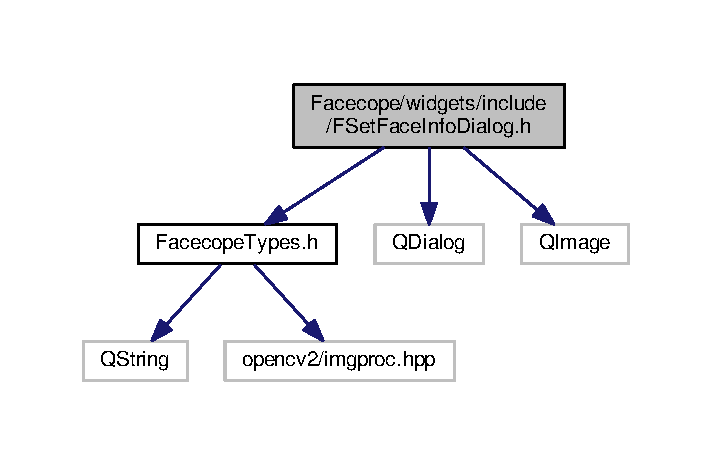
\includegraphics[width=342pt]{FSetFaceInfoDialog_8h__incl}
\end{center}
\end{figure}
\subsection*{Classes}
\begin{DoxyCompactItemize}
\item 
class \hyperlink{classFSetFaceInfoDialog}{F\+Set\+Face\+Info\+Dialog}
\end{DoxyCompactItemize}


\subsection{Detailed Description}
defines dialog for editing labels of face 


\hypertarget{FSettingsWidget_8h}{}\section{Facecope/widgets/include/\+F\+Settings\+Widget.h File Reference}
\label{FSettingsWidget_8h}\index{Facecope/widgets/include/\+F\+Settings\+Widget.\+h@{Facecope/widgets/include/\+F\+Settings\+Widget.\+h}}


defines settings-\/widget  


{\ttfamily \#include $<$Q\+Widget$>$}\newline
{\ttfamily \#include $<$Settings.\+h$>$}\newline
Include dependency graph for F\+Settings\+Widget.\+h\+:
\nopagebreak
\begin{figure}[H]
\begin{center}
\leavevmode
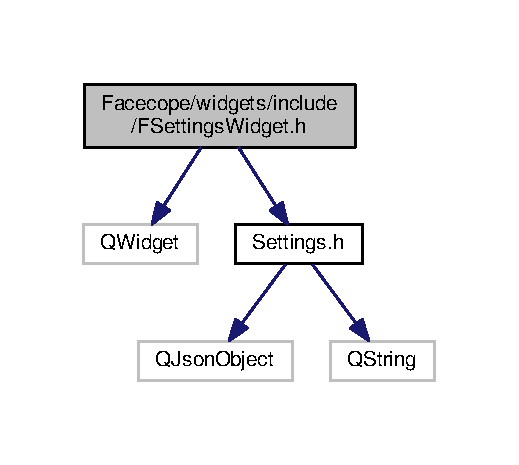
\includegraphics[width=249pt]{FSettingsWidget_8h__incl}
\end{center}
\end{figure}
\subsection*{Classes}
\begin{DoxyCompactItemize}
\item 
class \hyperlink{classFSettingsWidget}{F\+Settings\+Widget}
\end{DoxyCompactItemize}


\subsection{Detailed Description}
defines settings-\/widget 


\hypertarget{FWorkingWidget_8h}{}\section{Facecope/widgets/include/\+F\+Working\+Widget.h File Reference}
\label{FWorkingWidget_8h}\index{Facecope/widgets/include/\+F\+Working\+Widget.\+h@{Facecope/widgets/include/\+F\+Working\+Widget.\+h}}


defines main working-\/widget  


{\ttfamily \#include $<$F\+Image\+Proxy\+Model.\+h$>$}\newline
{\ttfamily \#include $<$F\+Main\+Facecope\+Model.\+h$>$}\newline
{\ttfamily \#include $<$Facecope\+Types.\+h$>$}\newline
{\ttfamily \#include $<$Q\+Completer$>$}\newline
{\ttfamily \#include $<$Q\+Drag\+Enter\+Event$>$}\newline
{\ttfamily \#include $<$Q\+Drop\+Event$>$}\newline
{\ttfamily \#include $<$Q\+File\+Info\+List$>$}\newline
{\ttfamily \#include $<$Q\+Image$>$}\newline
{\ttfamily \#include $<$Q\+List$>$}\newline
{\ttfamily \#include $<$Q\+Mutex$>$}\newline
{\ttfamily \#include $<$Q\+Size$>$}\newline
{\ttfamily \#include $<$Q\+Url$>$}\newline
{\ttfamily \#include $<$Q\+Widget$>$}\newline
{\ttfamily \#include $<$Settings.\+h$>$}\newline
Include dependency graph for F\+Working\+Widget.\+h\+:
\nopagebreak
\begin{figure}[H]
\begin{center}
\leavevmode
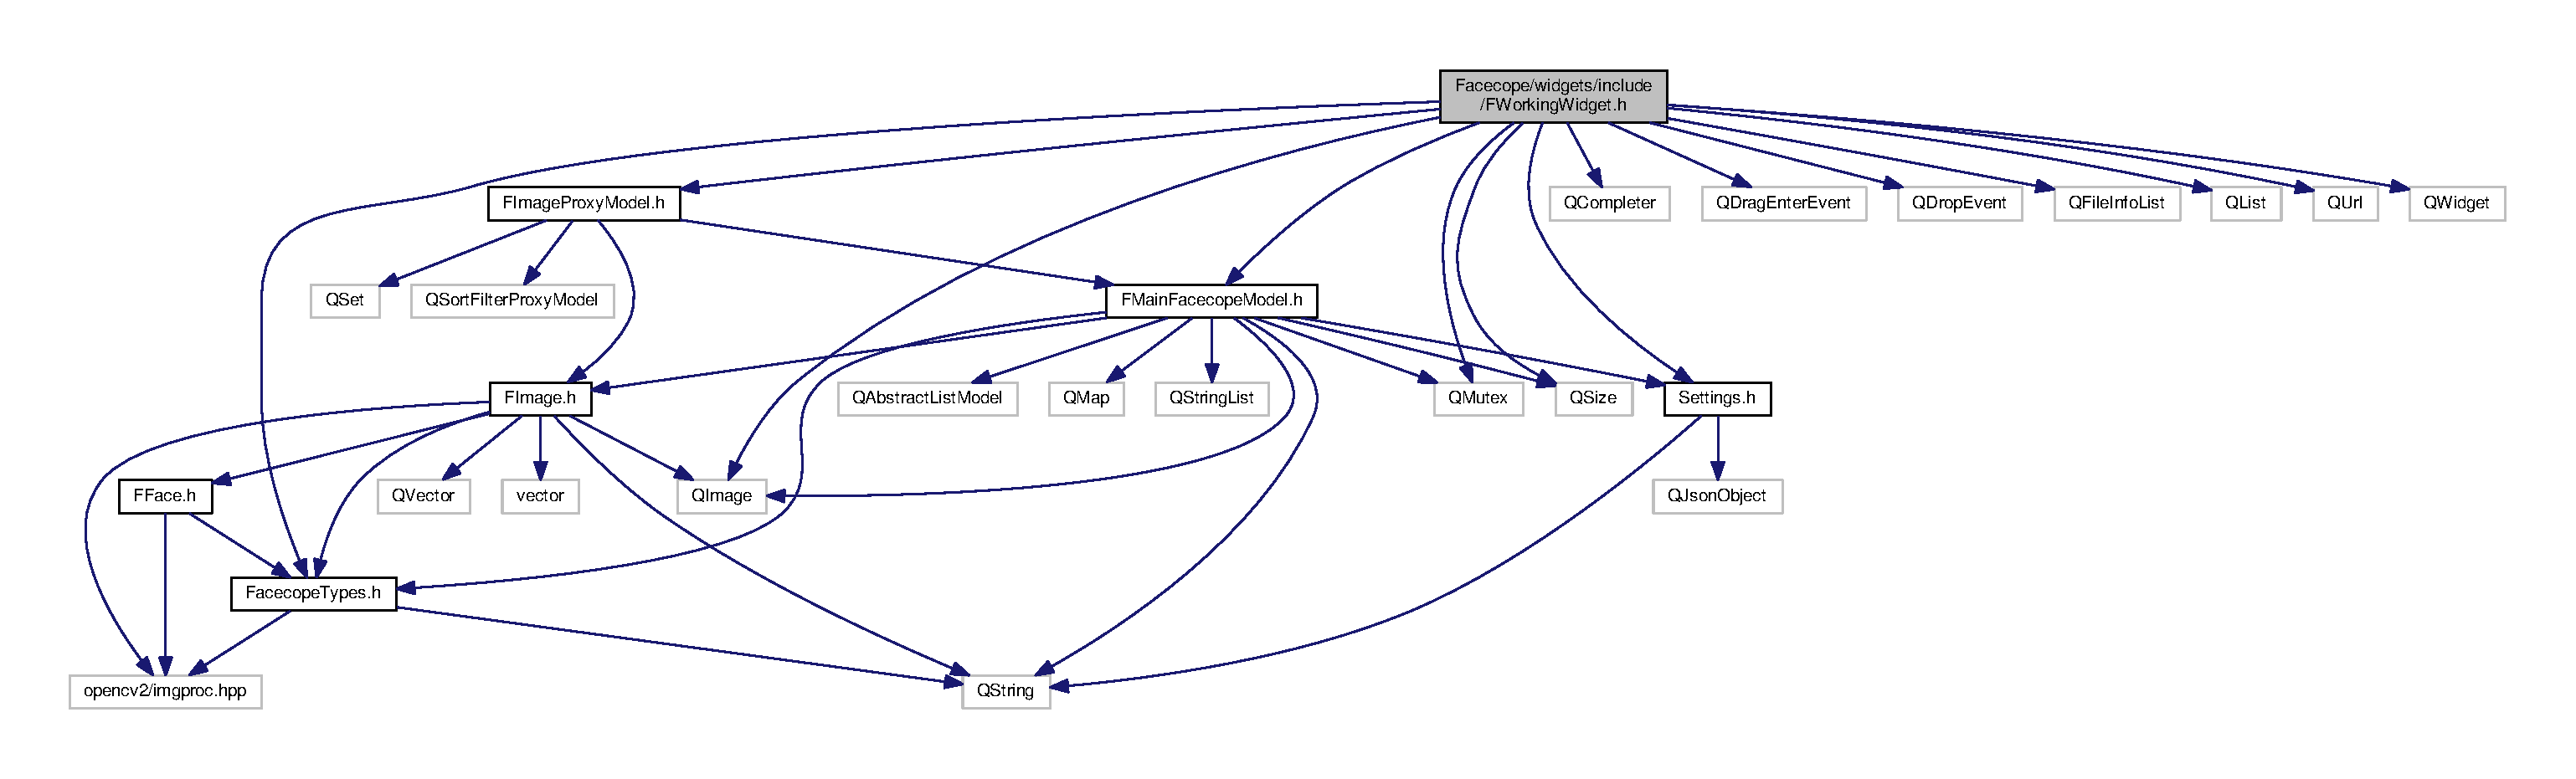
\includegraphics[width=350pt]{FWorkingWidget_8h__incl}
\end{center}
\end{figure}
This graph shows which files directly or indirectly include this file\+:
\nopagebreak
\begin{figure}[H]
\begin{center}
\leavevmode
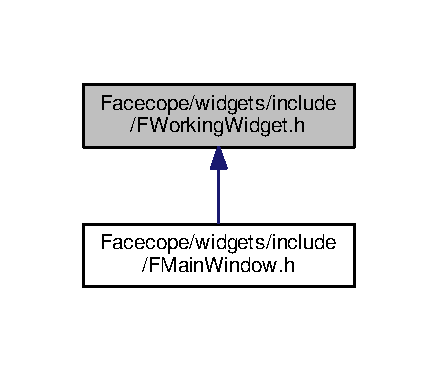
\includegraphics[width=210pt]{FWorkingWidget_8h__dep__incl}
\end{center}
\end{figure}
\subsection*{Classes}
\begin{DoxyCompactItemize}
\item 
class \hyperlink{classFWorkingWidget}{F\+Working\+Widget}
\end{DoxyCompactItemize}


\subsection{Detailed Description}
defines main working-\/widget 


%--- End generated contents ---

% Index
\backmatter
\newpage
\phantomsection
\clearemptydoublepage
\addcontentsline{toc}{chapter}{Index}
\printindex

\end{document}
